\chapter{Formalization of the semantic domain}
\label{Chap:HLFs}
Music Information Retrieval aims at designing automatic systems to help users visualize, browse, analyze and retrieve songs in large music collections. In Chapter \ref{Chap:LLFs} we formalized the musical content, which is the signal domain of the problem, by means of a feature representation; in this Chapter we formalize the high-level meaning of music, which is the semantic domain, by analyzing the so-called \textit{High-Level Features} (HLFs). 

The user semantics of music is affected by personal taste and users' background, and therefore there is a certain degree of subjectivity. When developing models for the formalization of music semantics, we assume there exists an objective baseline, i.e., an interpretation of the high-level meaning that is shared by the majority of people. We make use of this assumption as a constraint for the analysis of the semantic domain. This constraint can be later removed by designing approaches that consider users' customization.

In Section \ref{sec:HLFs:categorical} we discuss the most intuitive way to formalize the semantic domain, i.e., the \textit{categorical} approach. This approach represents the HLFs as a set of classes and classifies a given song with the HLFs that are feasible to describe it. The semantics of the set of classes, and therefore of the HLFs, can be disjoint or overlapping.

The former scenario, discussed in Section \ref{sec:HLFs:class} involves to classify a song into non-overlapping categories that fully describe a semantic characteristic of music. As an example, a given song can either be classified as \textit{vocal} or \textit{instrumental}, or as a \textit{live performance} or \textit{studio recording}. This kind of classification is helpful to create a major distinction between songs. Due to the complex nature of music, however, it is rare to find a set of strictly non-overlapping categories. As an example, the categories induced by the genre taxonomy are not disjoint, due to the existence of \textit{cross-genre} songs.

It is possible to overcome this issue by using overlapping HLFs, as discussed in Section \ref{sec:HLFs:anns}, where each HLF describe a high-level aspect of music and a song is formalized as the set of HLFs that are commonly used to describe it. Back to the example about genre, we formalize the semantic domain as a set of genre-related HLFs, and a given song is represented by the set HLFs that are used to describe it, such as \textit{rock}, \textit{pop}, \textit{glam rock}, etc. 

The categorical approach has two main limitations. The first limitation concerns its use for the description of entire songs, that therefore does not take into consideration the time-variance of music semantics. The same HLFs might not be able to describe different sections of the song. As an example, the song \textit{Live and Let Die} by Paul McCartney contains a slow and melancholic \textit{intro}, and a groovy and reggae \textit{bridge}. The second limitation concerns the low level of expressiveness of the categorical approach. In natural language, indeed, it is common to express not only whether a HLF describes a certain song, but also its degree of descriptiveness. The graded description allows people to compare songs, e.g., to describe a song as \textit{faster} or \textit{less stuttering} than another. 

We address the former limitation by formalizing the semantic domain of the musical \textit{structure}. This formalization, indeed, allows us to refer to the \textit{sections} within the song that are likely to be semantically uniform, i.e., time-invariant with respect to the high-level description. In Section \ref{sec:HLFs:MSA} we discuss how the structure is formalized in the state of the art.

The second limitation is addressed by formalizing the semantic domain following a \textit{dimensional} approach. This approach identifies the degree of descriptiveness of each HLF for a given song. Such graded description effectively increases the expressiveness of the model, providing an explicit and easy way to perform the aforementioned comparison between songs.

From a dimensional formalization of the semantic domain, we define a \textit{semantic model} as the model that embeds the dimensional HLFs. 
In Section \ref{sec:HLFs:models} we briefly discuss some dimensional semantic models proposed in the MIR literature. In a traditional semantic model, the HLFs are defined as independent with each other. In natural language, however, the terms are often semantically related with each other. In order to consider such relation in the model, we can include a \textit{semantic space} where the similarity among HLFs is defined, by means of two main approaches: by manually defining the model, the terms and the similarity among terms; or by automatically inferring the space from annotated data. 

In Section \ref{sec:HLFs:VA} we discuss the Valence-Arousal (VA) model as a specific case of a manually defined semantic space. The VA model is the main model for emotional-related descriptors and the mostly used in the music emotion recognition subfield. We also introduce the main dataset of HLFs that is collected for the VA model.

With regard to the automatically inferred semantic space, the main approach is based on the Latent Semantic Analysis (LSA) applied on large collection of annotated data.
An important source of data are the \textit{social tags} that are annotated directly by the users in the Internet. We discuss LSA and its application in MIR in Section \ref{sec:HLFs:LSA}.

The two approaches are treated as mutually exclusive: either the semantic space is manually defined or it is automatically inferred. In this regard, in Section \ref{sec:HLFs:ANEW} we investigate a hybrid approach to improve a manually defined semantic space by including information that is inferred from annotated data. We focus on the Valence-Arousal model using LSA-based or manually collected information. This approach also contributes to enrich the defined space with some context specific to the music description scenario. This study was presented at the International Conference for Music Information Retrieval (ISMIR) \cite{Buccoli2016AHE},

For the sake of completeness, in Section \ref{sec:HLFs:ontology} we provide an overview of the most advanced formalization of the semantic domain, i.e., the ontologies, which aim at modeling the complete domain of knowledge of a given subfield.%, so  the state of the art is still in a beginning stage.

%The common approach to address music annotation is to define a set of HLFs for the semantic domain and use them to describe a music item with the set of meaningful HLFs.
%
%
%Consequently, the classification is frequently based on multiple, overlapping categories, that need to address several categories. 
%
%In order to do so, we define a set of HLFs, or \textit{tags}, that are used to model the semantic domain
%
%We can first refer to a semantic description that is close to the musical content, by considering the Music Structure Analysis (MSA), which concerns the identification of the segments within the song that can be grouped into categories named \textit{sections} based on their content. In Section \ref{sec:HLFs:MSA} we discuss how MSA provides a well defined and objective formalization for the semantic domain. 
%
%
%Two are the main approaches for the formalization of the semantic domain: the categorical approach and the dimensional approach. The former, described in Section \ref{sec:HLFs:categorical}, ; the latter, described in Section \ref{sec:HLFs:models}, identifies the degree of descriptiveness of a HLF for a music item.



%design a solving algorithm to automatically infer the classification for the descriptors within the set. 




%In the following we present the state of the art of the formalization of the semantic domain. We also provide a theoretical background on some tasks that are more relevant for this work. 




\section{Categorical description of music}\label{sec:HLFs:categorical}
\subsection{Disjoint classes}\label{sec:HLFs:class}
Due to the complexity and variety of the music semantics, the disjoint categorization of music is rather rare. Nevertheless, it has been addressed by the MIR community by constraining more general cases. An example is the case of classifying a song by performing artist. While different artists can perform the same song (the main and the \textit{featuring} artist), \cite{mandel2005song} presents an approach for artist identification obtained by composing a dataset of 1200 pop songs by a subset of 18 artists. In \cite{Bestagini2013b} the use-case of music classification between \textit{official live performances} and \textit{unofficial bootleg recordings} is discussed. The classification is made possible by composing the dataset with songs from only these two categories. In Chapter \ref{Chap:Bootleg} we analyze the complete scenario by adding the official studio recording category.

%cerca A Survey of Audio-Based Music Classification and Annotation

Some simple case of music emotion and genre recognition falls into the disjoint categorization. While the semantics of emotion is very rich and complex, and discussed in detail in Section \ref{sec:HLFs:VA}, some constraints can be added in this task. A common approach is to divide the emotion spectrum into a set of categories and then classify the emotional content of each song into one of these categories. In \cite{Hu:2007} the authors define five clusters for emotion-related descriptors: 
\begin{itemize}
\item \textbf{Cluster 1} Rowdy, Rousing, Confident, Boisterous, Passionate;
\item \textbf{Cluster 2} Amiable/Good natured, Sweet, Fun, Rollicking, Cheerful;
\item \textbf{Cluster 3} Literate, Wistful, Bittersweet, Autumnal, Brooding, Poignant;
\item \textbf{Cluster 4} Witty, Humorous, Whimsical, Wry, Campy, Quirky, Silly;
\item \textbf{Cluster 5} Volatile, Fiery, Visceral, Aggressive, Tense/Anxious, Intense.
\end{itemize}
%Cluster_1: passionate, rousing, confident,boisterous, rowdy
%Cluster_2: rollicking, cheerful, fun, sweet, amiable/good natured
%Cluster_3: literate, poignant, wistful, bittersweet, autumnal, brooding
%Cluster_4: humorous, silly, campy, quirky, whimsical, witty, wry
%Cluster_5: aggressive, fiery,tense/anxious, intense, volatile,visceral
These five clusters are used as a reference for several works on emotion classification \cite{Bischoff:2009, laurier2008multimodal, Laurier2009}.

The same approach is used for the formalization of semantics regarding the music genre: instead of addressing the complete and highly complex scenario of genre representation, some macro non-overlapping genres are defined and used as reference. In \cite{tzanetakis2002musical} the authors present a dataset for musical genre recognition base on a set of 10 genre descriptors: \textit{Blues}, \textit{Classical}, \textit{Country}, \textit{Disco}, \textit{Hip Hop}, \textit{Jazz}, \textit{Metal}, \textit{Popular}, \textit{Reggae}, and \textit{Rock}. This dataset has been used as a benchmark for genre recognition by a wide part of the community \cite{Sturm2012GTZAN}. In \cite{Scaringella2006} the defined genre are, instead, \textit{classical}, \textit{ambient}, \textit{electronic}, \textit{new-age}, \textit{rock}, \textit{punk}, \textit{jazz}, \textit{blues}, \textit{folk}, and \textit{ethnic}. This set of genres are effectively used as a broad categorization of musical content or as a constrained use-case to test real application scenarios. However, they are special or limited case that need to be eventually expanded.
%
\subsection{Overlapping categories}\label{sec:HLFs:anns}
In the categorical approach, the semantic domain is formalized as a set of multiple, independent HLFs, where each descriptor is only used or not used for the description of a song. It can be seen as a multi-label classification problem, where each classification concerns the presence or absence of a descriptor in a song. %More formally, instead of having one $N$-category classification, the music annotation concerns $N$ two-category classifications.

In \cite{wordsCAL500}, the authors define a set of 159 HLFs spanning several semantic aspects of music:
\begin{itemize}
\item \textit{emotion}: concerns feelings inspired by the songs; 
\item \textit{genre}: the musical genre of the songs;
\item \textit{instrument}: the instruments played during the song, including \textit{male} and \textit{female lead vocals};
\item \textit{song}: some high-level properties of the song, such as \textit{changing energy level}, \textit{catchy/memorable} ; 
\item \textit{usage}: typical situation for listening that particular song e.g., \textit{at a party}, \textit{going to sleep} and so on);  
\item \textit{vocals}: the style or features of the singer, such as \textit{duet} or \textit{breathy}.
\end{itemize}
This set of descriptors, together with the collected dataset described in \cite{Turnbull2007} (CAL500), have been widely used in the community for the task of music annotation \cite{coviello2011, nam2012learning,yeh2014improving}. The descriptors are treated as independent, while a strong correlation among them is highlighted by \cite{Miotto2012}, who suggest a generative model to exploit it.

A valuable source of information for music annotation is provided by the social tags. The \textit{tags} are free-text labels that are largely used in blogs, forum and social networks (as \textit{hashtags}) to classify content. They have been extremely used for music description as well, providing a tremendous amount of information for music researchers \cite{lamere2009}. In particular, the Internet web service Lastfm\footnote{www.lastfm.com} contributed to create and made available a large dataset of tagging information. Social tags can help to formalize the semantic domain with the categorical approach, with an amount of tags that is close to the number of words used in the natural language. The collection of tags from multiple users has been named \textit{folksonomy}, a taxonomy from the folk \cite{morrison2008tagging}. The social tags present several issues: the data is not structured and noisy, e.g., for different spelling (e.g., \textit{rock}, \textit{rock'n roll}, \textit{rock and roll}); the tags reflect the semantics of the users, so they include a certain degree of subjectivity;  each user follows their taste while tagging and it is hard to understand whether a certain tag describes the content of the music or a judgment by the tagger; malicious tags can be generated in the worst case scenario. Moreover, popular songs receive more annotations and tags, while less popular ones are likely not to be annotated \cite{lamere2009}. 
Nevertheless, the social tags have been extensively exploited by MIR researchers as a source of information and a definition of the semantic domain \cite{Celma2008,eck2008automatic,begelman2006automated,Levy2007}.

%The multi-label approach used in music annotation helps to formalize the semantic domain, since a. 
The  categorical approach is sufficient to formalize the semantic domain for several simple use-cases. However, this approach is not able to fully describe the semantics used for music, since it cannot model the intensity in the description. While the intensity might in fact be coded into the meaning of words, this strategy would implicitly rely on the objectivity of the words' semantics and on an extremely large set of descriptors. For this reason, in Section \ref{sec:HLFs:models} we discuss the dimensional approach, which leads to a simpler explicit modeling of the intensity.



\begin{figure}[tbp]
	\begin{center}
		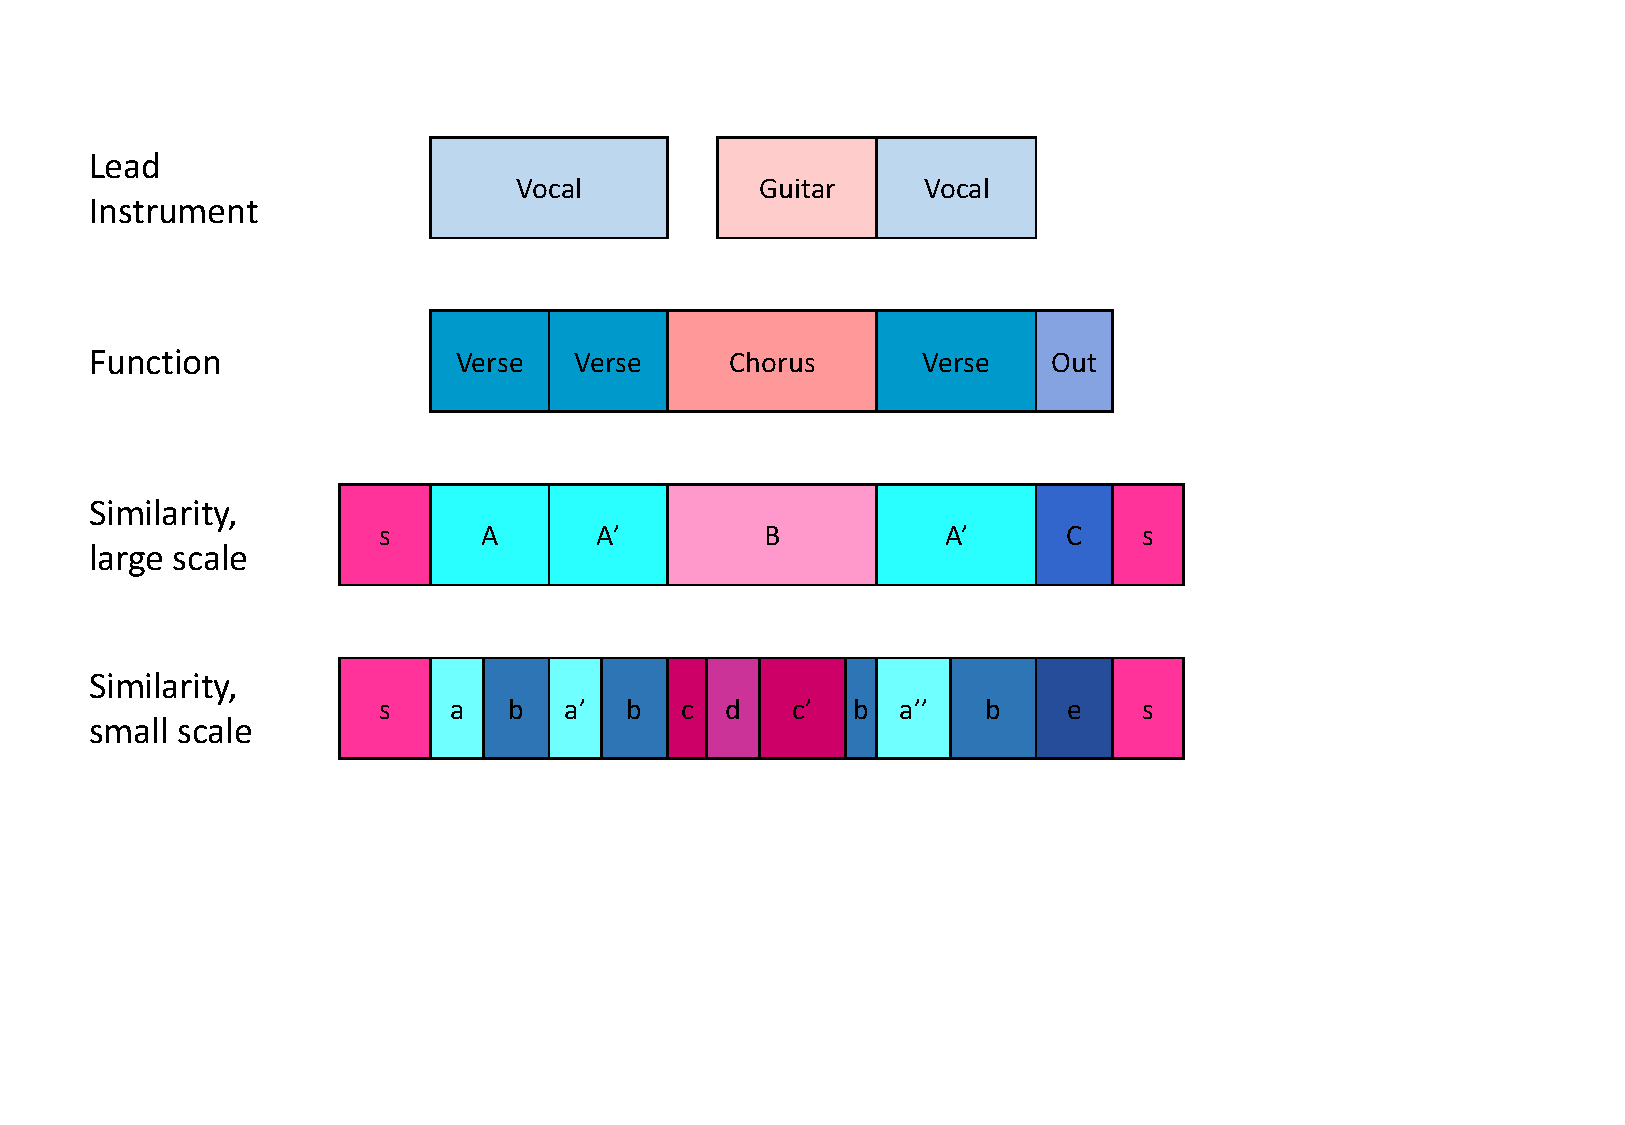
\includegraphics[trim=1cm 6cm 6cm 2cm,clip=true,width=\textwidth]{img/HLFs/functionColors}
		%\psfig{file=img/ML/logopm.jpg,width=3.5cm}
	\end{center}
	\caption{Example of the different labeling proposed in \cite{Smith2011}}
	\label{fig:HLFs:MSAscales}
	
\end{figure}

\section{Musical Structure Analysis}\label{sec:HLFs:MSA}
We infer useful information from the structure of a song, and the structure itself is in fact a high-level representation of it. In \cite{Smith2011} the authors present the dataset SALAMI, that is composed of structural annotations for around 1400 musical recordings. The authors also introduce several paradigms for the structural annotation (see Figure \ref{fig:HLFs:MSAscales}), that can be seen as structure-based HLFs:
\begin{enumerate}
	\item \textit{Lead Instrument} to identify the section based on the lead instrument (Vocal, Guitar, etc.);
	\item \textit{Function} to identify the section based on the semantic function, drawn from a set of 20 labels (see Table \ref{tab:HLFs:MSAfunctions});
	\item \textit{Similarity, large scale} does not add a semantics, it just uses letters to identify the sections. Similar sections, like two verses, are identified by the same letter;
	\item \textit{Similarity, small scale} focuses on shorter sections to identify them; the boundaries of the large scale match some of those in the small scale.
\end{enumerate}

The semantic domain for the problem of automatic MSA is particularly well formalized. However, automatic approaches perform only the boundary detection and grouping of similar sections, without annotating the song with the label \cite{ullrich2014boundary,Nieto2D,Nieto2016,NietoCNMF}, so the semantic domain in this case is not fully exploited. Moreover, the linking function from the signal domain is still not clear, as discussed in Section \ref{sec:ML:MSA}. We address the problem in Chapter \ref{Chap:MSA}.

\begin{table}[tbp]
\caption{List of labels for function-based MSA}
\label{tab:HLFs:MSAfunctions}
	\centering
	\large
	\bgroup
	\def\arraystretch{1.5}
	\begin{tabular}{||p{.25\textwidth}|p{.7\textwidth}||}
		\hline
		\hline
		\textbf{Group} & \textbf{Labels} \\
		\hline
		\hline
		Basic group & intro, verse, chorus, bridge\\
		\hline
		Instrumental & instrumental, solo\\
		\hline
		Transition & transition, pre-chorus, pre-verse, interlude\\
		\hline
		Genre-specific & head, main theme, (secondary) theme\\
		\hline
		Form-specific & exposition, development, recapitulation\\
		\hline
		Ending & outro, coda, fadeout\\
		\hline
		Special labels & silence, end\\
		\hline
		\hline
	\end{tabular}
\egroup

\end{table}

 \begin{figure}[tbp]
    \begin{center}
      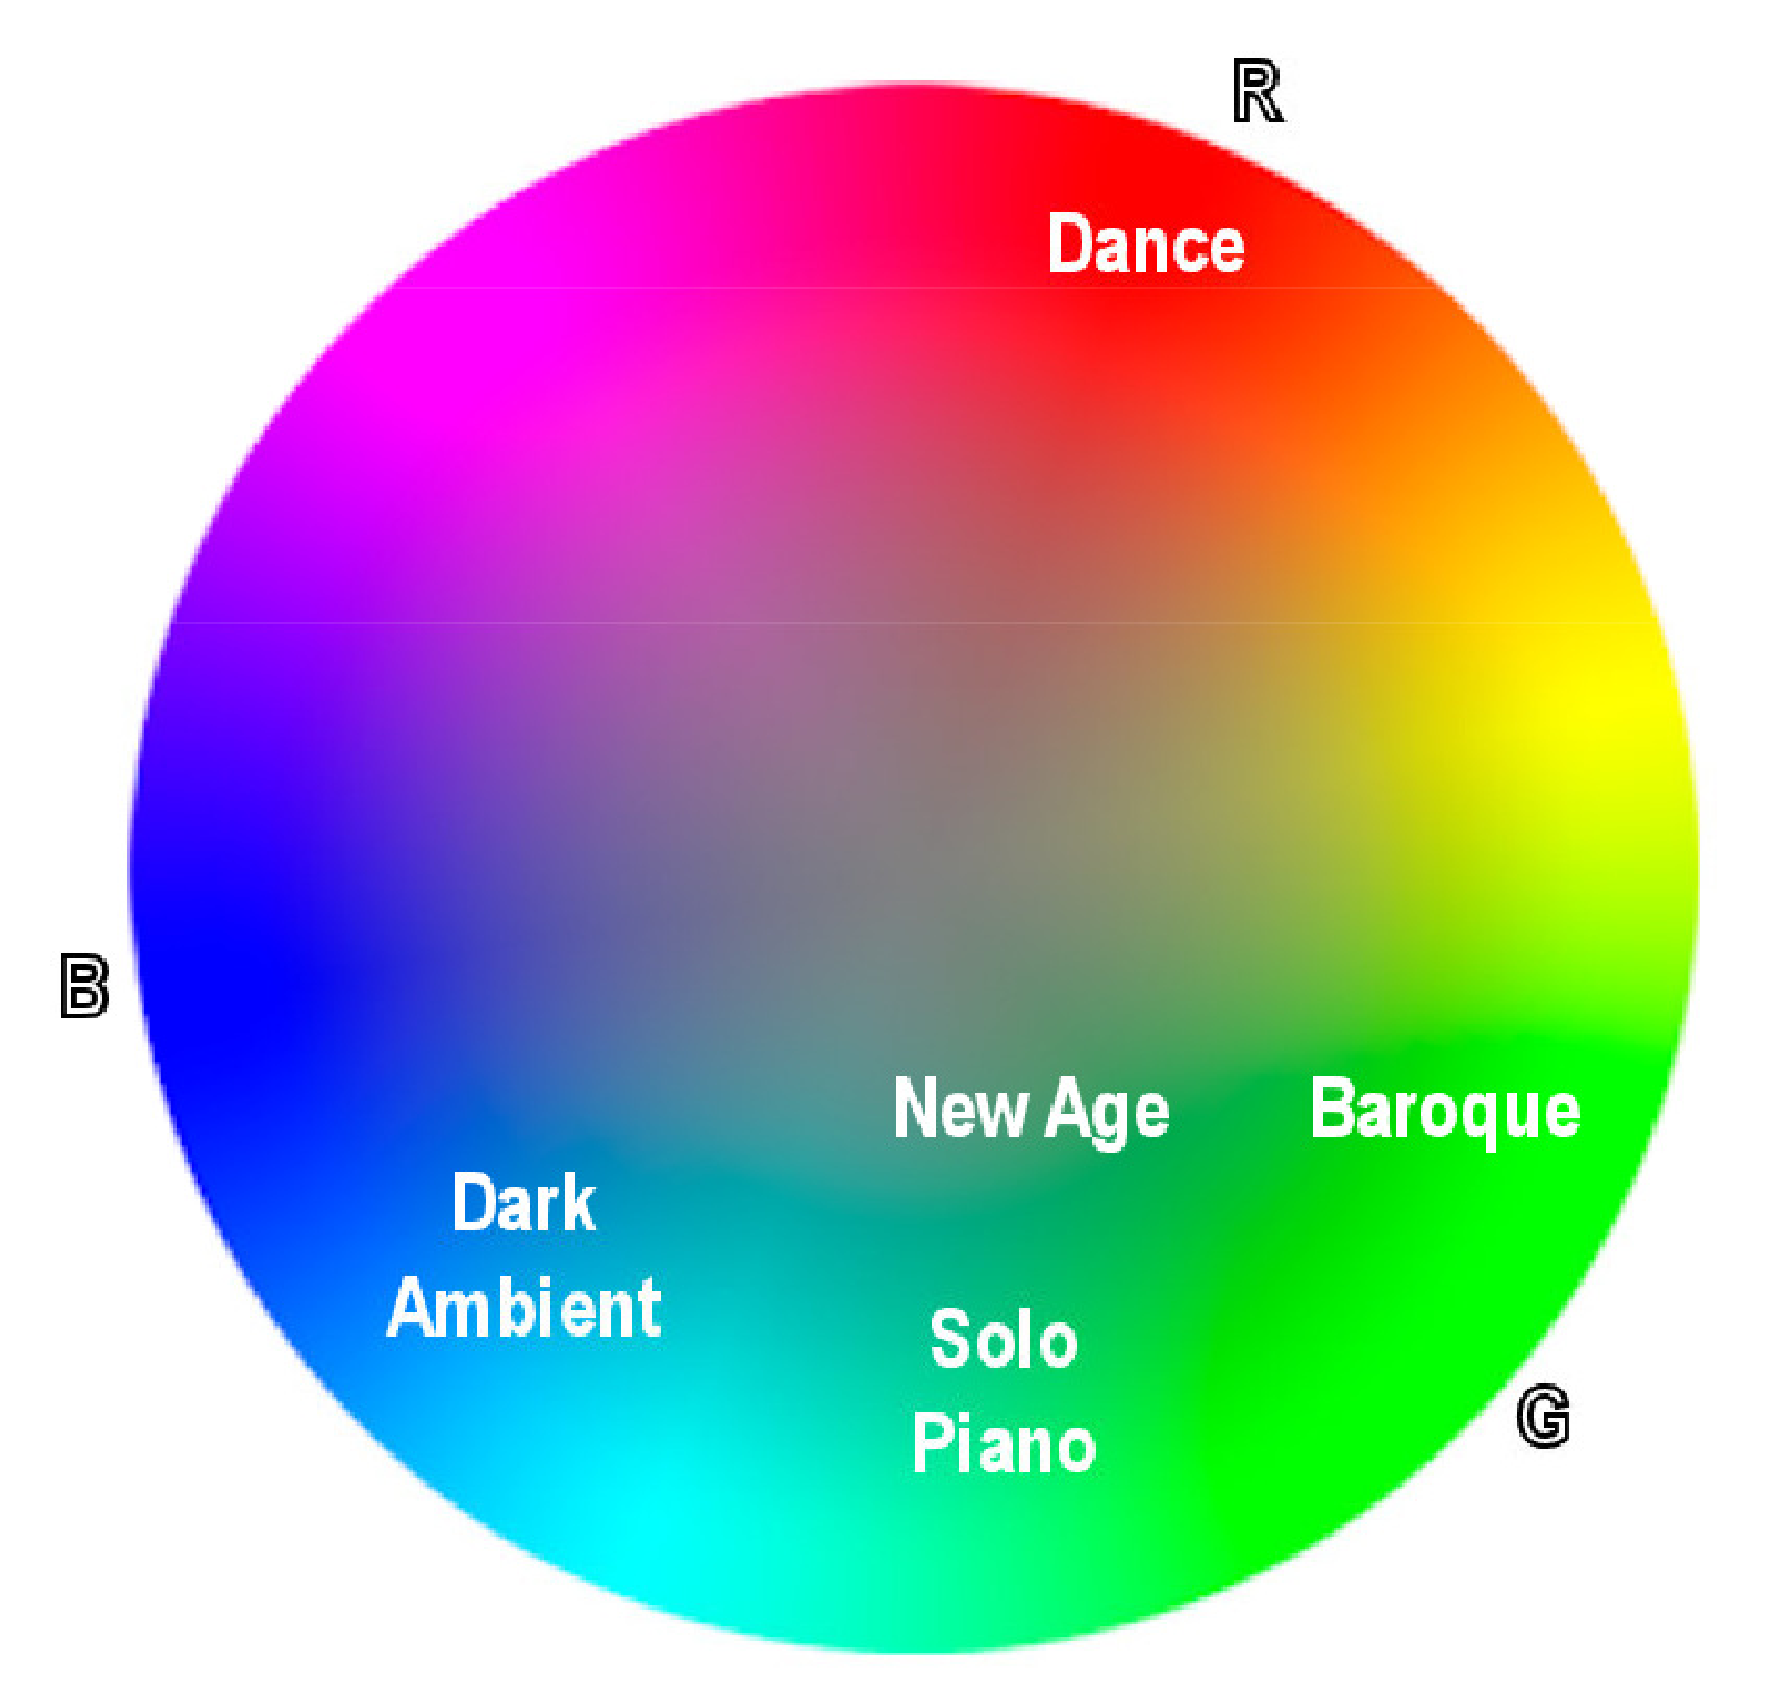
\includegraphics[width=8.5cm]{img/HLFs/triangleB}
	%\psfig{file=./pictures/logopm.jpg,width=3.5cm}
    \end{center}
  \caption{The 3D genre visualization from \cite{Prandi2009}}
  \label{fig:HLFs:prandi}
  \end{figure}


\section{Dimensional description of music and semantic models}\label{sec:HLFs:models} %dimensional}
%\subsection{Semantic Models}\label{sec:HLFs:models}
A dimensional semantic model concerns the use of a set of dimensional high-level descriptors, which allow to express the intensity of the description by using a continuous range of values. 

In \cite{Prandi2009} the authors identify three dimensional HLFs to represent music genres: \textit{darkness}, \textit{dynamicity} and \textit{classicity}. They use the three descriptors to span a 3D music genre space, where each genre is an area in the space, and areas can overlap. The three dimensions are also associated with the three basic color to design a visualization tool, as shown in Figure \ref{fig:HLFs:prandi}. 

In \cite{Buccoli2013} the authors propose a set of 9 bipolar dimensional HLFs to describe non emotional-related aspects of music: \textit{soft/hard}, \textit{clear/dull}, \textit{rough/harmonious}, \textit{void/compact}, \textit{flowing/stuttering}, \textit{dynamic/static}, \textit{groovy/not groovy}, \textit{easy/difficult} and \textit{fast/slow}. The non-emotional related content is represented in the model with a numerical value for each of the descriptor, and the HLFs are defined as independent with each other.

%The authors do not populate the model with terms, nor they define a semantic distance among descriptors, but the dimensionality of the model allows to define the intensity of the descriptors by using qualifiers from \cite{LIKERT} (e.g., \textit{moderately groovy}, \textit{extremely difficult}) and to define a semantic similarity metric between the representations of the songs.

A semantic model is refined by defining not only the set of descriptors, but also the semantic relations among them. Such semantic similarities are either manually designed or automatically inferred. With the former approach, a set of descriptors is chosen and some explicit or implicit semantic distance between them is defined. In Section \ref{sec:HLFs:VA} we discuss the most popular example of this approach, i.e., the Valence-Arousal semantic model for emotion representation. With the latter approach, some numerical or algebraic algorithms are applied on a set of data in order to infer a similarity metric. Several researchers have employed the Latent Semantic Analysis with this aim, so we discuss this approach in detail in Section \ref{sec:HLFs:LSA}.

 \begin{figure}[tbp]
    \begin{center}
      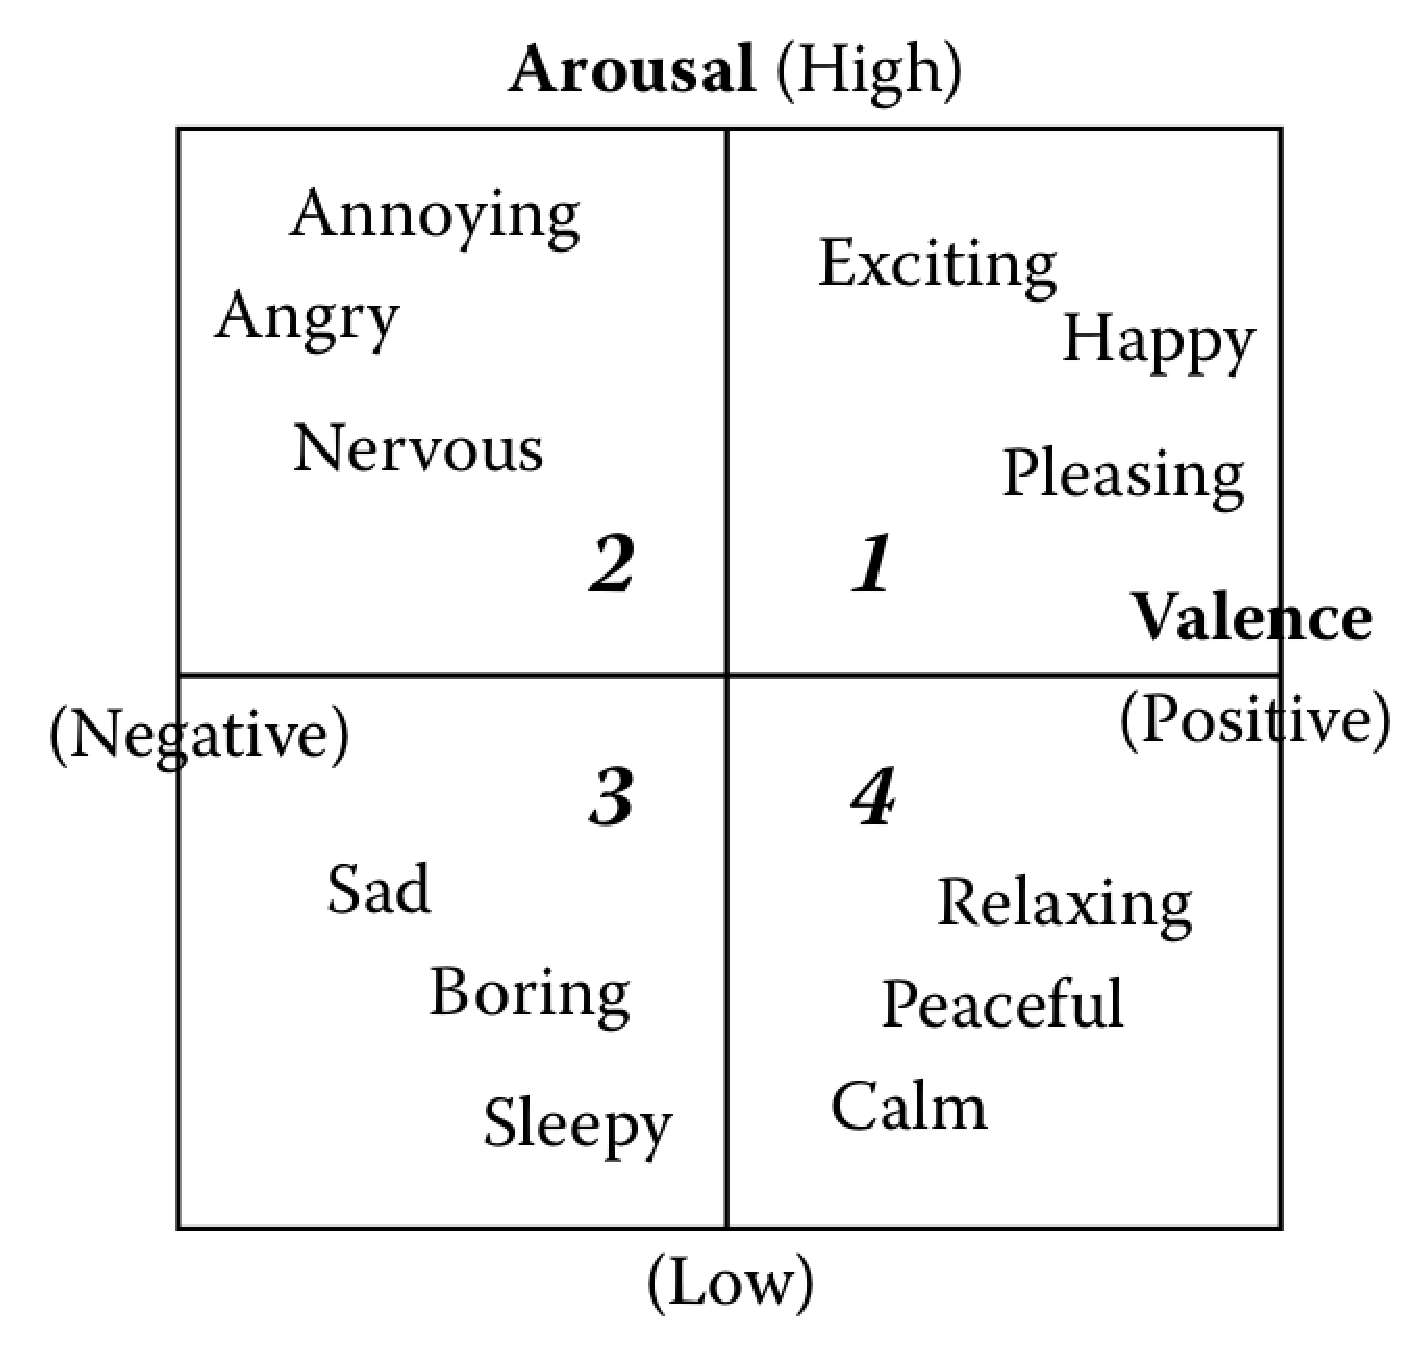
\includegraphics[width=8.5cm]{img/HLFs/VAmoods}
	%\psfig{file=./pictures/logopm.jpg,width=3.5cm}
    \end{center}
  \caption{The 2D Valence-Arousal emotion plane, with some emotional-related descriptors approximately mapped \cite{Yang2012}}
  \label{fig:HLFs:VAmoods}
\end{figure}

\subsection{The Valence-Arousal Model}\label{sec:HLFs:VA}
One of the fundamental properties of music is the ability to convey emotions\cite{Yang2012}. Consequently, the Music Information Retrieval community has been greatly interested in representing and classifying music according to emotions for music recommendation and personalization \cite{Barthet2012, Juslin:2001, Juslin2011, Lee2004, Yang2012}. Traditional meta-tags like artist or title are not informative on the content of a music piece and several studies \cite{Juslin:2001, Juslin2011, Lee2004, Yang2012} on user needs and behaviors have proven, in fact, the interest of representing and classifying music according to emotions. 

It has been proven, indeed, that listeners enjoy looking for and discovering music using emotion-based queries, which represents 33\% of music queries according to \cite{Lee2004}. This is an important reason that urged music psychologists and musicologists to investigate different paradigms for the representation and modeling of emotion related descriptors \cite{Juslin:2001, Juslin2011, Lee2004}. In \cite{Barthet2013} the authors review a high number of categorical and dimensional semantic models for music emotion recognition, including the one proposed in \cite{Russell1980}.

In \cite{Russell1980}, the authors propose a semantic model of emotions based on two dimensional descriptors, the Valence and the Arousal. The Valence indicates the graded polarization of the sentiment, from negative to positive, whereas Arousal estimates the degree of energy, or activation, in the emotion, from low to high. Emotional-related descriptors are modeled as a combination of Valence and Arousal and represented in the 2-dimensional VA space. The dimensional space allows a continuous shading of the formalization of the semantics of emotions, with some well defined areas such as represented in Figure \ref{fig:HLFs:VAmoods}: 
\begin{itemize}
\item joyful emotions are represented in an area with high arousal and positive valence; 
\item sad emotions are assigned with low arousal and negative valence;
\item aggressive emotions are represented in the high-energy, negative-valence portion;
\item calm emotions are defined as low arousal and positive valence sample.
\end{itemize}

The VA model can be used for mapping both HLFs and music (or any other) content. Since the VA model defines a dimensional space, a metric distance can be defined in order to model the semantic distance among descriptors, among the representation of the content, or even between descriptors and content. Given two generic items in the VA space $\mathbf{x}=[x_V,x_A]\T $ and $\mathbf{y}=[y_V, y_A]\T$, a simple distance metric is the Euclidean distance:
\begin{equation}
d(\mathbf{x},\mathbf{y})=\sqrt{(x_V-y_V)^2+(x_A-y_A)^2}.
\end{equation}

\begin{figure}[bt] 
	\centering 
	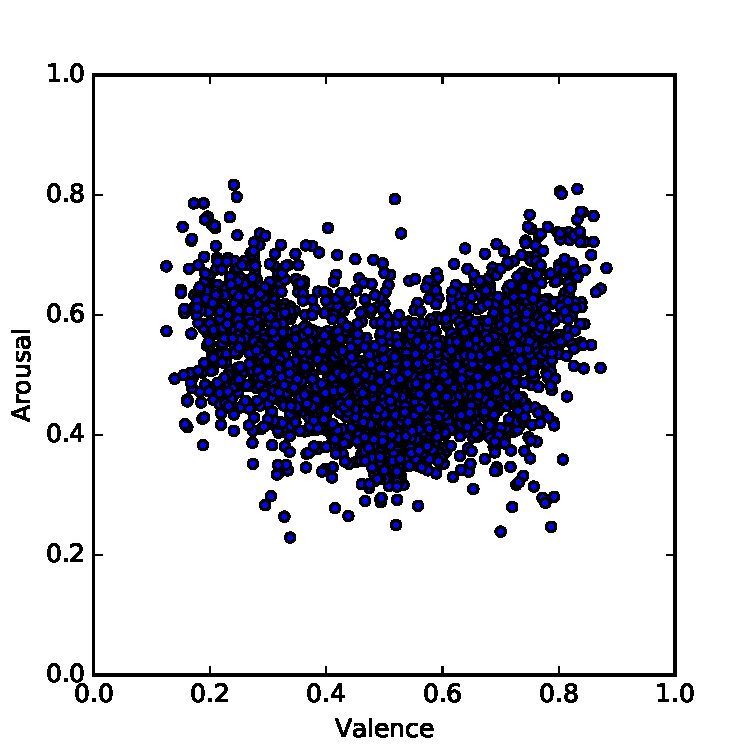
\includegraphics[width=0.75\columnwidth]{img/ANEW/ANEW.pdf}
	\caption{Distribution of the ANEW dataset in the VA space}
	\label{fig:HLFs:ANEW}
\end{figure}	

Some works propose a third dimension for the VA model \cite{Kim2010}, but no agreement has been reached within the community yet. While a third dimension potentially increases the precision of the model, it also increases its complexity and the cognitive load required for annotation. In \cite{bigand2005multidimensional} the authors propose a third dimension to represent the continuity or discontinuity of the emotion, or the melodic-harmonic contrast for music-related emotion description. In \cite{scherer2004emotions} the third dimension is identified as the \textit{dominance} (D), which expresses the degree of control of the emotion. Dominance allows to distinguish possibly overlapping emotions, such as fear and anger, that are both negative and active. While the VA space is more widely used \cite{Weninger2014, aljanaki2015emotion}, the Valence - Arousal - Dominance (VAD) space has received some attention as well \cite{Yang2012, Cowie2012, Scherer2004}. 

The increasing need of a continuous affective model led to the creation of the \textit{Affective Norm for English Words} (ANEW) dataset \cite{Bradley1999} for psychological research. This dataset is composed of 2,476 English words with positions in the VAD space. Albeit it is a generic dataset, the large amount of terms in ANEW makes it a powerful resource also for the Music Emotion Recognition (MER) community, including applications for automatic music annotation and retrieval \cite{Buccoli2013, Saari2015}. Unfortunately, ANEW terms in the VAD space tend to have a very uniform and compact distribution concentrated around the center of the space as shown in Figure \ref{fig:HLFs:ANEW} for the VA projection. 

Although the use of a substantial set of terms provides a very representative model of a large variety of emotions, to deal with a compact and cluttered distribution can be problematic in many musical applications. For this reason, typically only a subset of the terms is used, leading to a loss in the exhaustiveness of the model. In the following Section \ref{sec:HLFs:ANEW} we discuss the improvement of the ANEW dataset by adding annotations on the music semantics of the HLFs. Such annotations are, in fact, also automatically inferred by means of a Latent Semantic Analysis, which is described in the next Section.

\subsection{Latent Semantic Analysis}\label{sec:HLFs:LSA}
The semantic annotation scenario pictured in Section \ref{sec:HLFs:anns} defines the semantic domain, but it does not model the semantic relation among the descriptors. This issue is common in other information retrieval scenarios and has been addressed by generating a semantic space from annotated dataset, by means of Latent Semantic Analysis (LSA).

Given a dataset of items annotated with several HLFs, LSA builds a semantic model by inferring graded similarities among descriptors from the frequency with which they are used together in the annotation of items (\textit{co-occurrence}). As an example, if the descriptors \textit{quiet} and \textit{calm} are frequently used together and on the opposite, \textit{quiet} and \textit{aggressive} never co-occur, the LSA can infer that \textit{quiet} and \textit{calm} are highly similar, while \textit{quiet} and \textit{aggressive} are more likely to be opposite. More formally, the LSA is based on the approximation of the matrix that collects the annotations. Such an approximation is able to exploit the relations among the HLFs and among the tracks, leading to a novel vector space where each basis vector is a linear combinations of the original descriptors. The HLFs are therefore represented as a linear combination of the novel basis vectors, and the distance between such representations is related to the semantic relations of the underlying concepts \cite{Manning2008}. In Section \ref{app:LSA} we provide the technical background of the LSA.

In order to build a reliable semantic model, it is required to have access to a large annotated dataset. This is the reason why LSA has been effectively used with annotation from social tags, that collect annotations from thousands of users, for thousands of songs, with thousands of descriptors \cite{lamere2009}.

LSA-based approaches have been often employed by MIR community to derive semantic models from large annotated dataset. In \cite{Levy2007} the authors use tags collected from the last.fm and MyStrands web services to build a generic semantic space. In \cite{Celma2008} the author infers a dimensional space with LSA and exploits such novel space to define a metric of semantic similarity among annotated tracks. The works described in \cite{Laurier2009,saari2014semantic} focus on a semantic space for emotional-related descriptors and apply the LSA to obtain a lower-dimensional space for the HLFs. In particular, the authors of \cite{Laurier2009} compare the obtained space with the Valence-Arousal model, while the authors of \cite{saari2014semantic} apply multidimensional scaling to compute an automatic mapping from the LSA-based emotional-related HLFs to the Valence-Arousal space.

Although the LSA is a powerful resource to automatically define the semantic domain by means of a dimensional model, its use might rises some issues related to its use. First, the quality of annotations is crucial in this task, and social tags are often a noisy and unreliable source of information. Moreover, the LSA assumes that the co-occurrence of descriptors is related to their similarity, which is not always true. Finally, the phenomenon of \textit{polysemy}, i.e., a term with several meanings, is common in the natural language, and it is hard for LSA to infer the different meanings, which lead to different similarities among HLFs. In Chapter \ref{Chap:DCSM} we define a semantic model that can deal with different contexts, as sub-models, to address the issue of polysemy.

%

\section{An exploration of the semantic domain for emotional-related description}\label{sec:HLFs:ANEW}
In Section \ref{sec:HLFs:VA} we presented the Valence-Arousal (VA) model, which is one of the most widely used semantic model for the representation of emotional-related descriptors and content. The Valence is linked to the degree of pleasantness, while the Arousal represents the degree of excitement, or activation. A third dimension, related to \textit{Dominance} (D), is sometimes added to express the degree of control and to possibly distinguish different and overlapping emotions \cite{Cowie2012, Scherer2004}, leading to the Valence, Arousal, Dominance (VAD) space. In Section \ref{sec:HLFs:VA} we also discussed about the \textit{Affective Norm for English Words} (ANEW) dataset \cite{Bradley1999}, which is composed of almost 2,500 emotional-related descriptors mapped in the VAD space. While the dataset has been a helpful resource for the MIR community, it was not specifically designed for music description, and therefore its use presents some difficulty related to the distribution of terms and to the semantic relation among terms. As an example, it is not sure whether the metric of distance defined in the VA/VAD space can match the semantic similarity for the context of music description. Moreover, due to the clutter distribution of terms (see Figure \ref{fig:HLFs:ANEW}) it is difficult to conceptually organize them into a  hierarchy that is closer to how people describe music.

% \begin{figure}[bt] 
%   \centering 
%   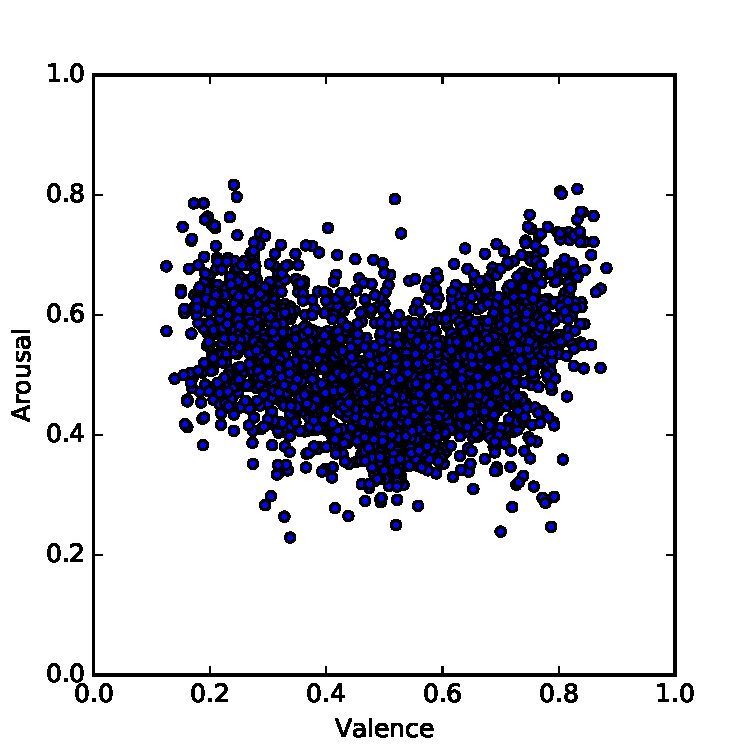
\includegraphics[width=0.9\columnwidth]{img/ANEW/ANEW.pdf}
%   \caption{Distribution of the ANEW dataset in the VA space}
%   \label{fig:ANEW:ANEW}
% \end{figure}  


%In this scenario, the domain and the codomain of the problem both lie in the semantic world, and we aim at finding a linking function that is able to shape the VA or VAD semantic model to the novel space.

In this Section, we investigate the production of a novel emotional space, where the terms from ANEW dataset are better conceptually organized and bear more relevance for music description. Such emotional space would be highly helpful for the development of novel music application that rely on high-level emotional-related descriptors. In this study we build the new emotional space by taking advantage of kernel expansion techniques applied to the VA and VAD space, in order to design higher-dimensional emotional spaces.  Although the kernel transformation has the effect to produce a more sparse distribution of terms, it is not clear if the  semantic distance between concepts is well represented by the metric in the new space. We then use the prior information on music description to find a distance reflecting conceptual organization of terms by applying distance learning techniques \cite{xing2003distance, bar2003learning, goldberger2004neighbourhood}, as discussed in Section \ref{sec:ML:dist}. Given some constraints between terms, these methods search for a linear transformation of the space that is semantically relevant. That is, the ideal learned distance closely correlates with semantic differences given by users in a specific task for a subset of the ANEW terms. 

We generate the set of constraints using ``a priori'' information collected through a subjective test where participants were asked to specify the semantic similarity between pairs of terms in the context of music. We then perform Latent Semantic Analysis on emotion related annotations for a large set of music pieces. 

Under the hypothesis that the position of the terms in the space may be improved by this transformation, we validate the approach by grouping (i.e.,  clustering) the descriptors in the new high-dimensional space. In order to isolate the effect of distance learning from the use of apriori constraints, we use both unsupervised clustering techniques and semi-supervised clustering techniques. The latter make use of the same kind of constraints to retrieve the clusters with more relevance to the music semantics. We subsequently evaluate the resulting clusters with objective and subjective metrics. Tests show promising results given these new learned distance metrics and provide an insight into how a better configuration in the high-dimensional space can be achieved. 


 \begin{figure}[tb] 
  \centering 
  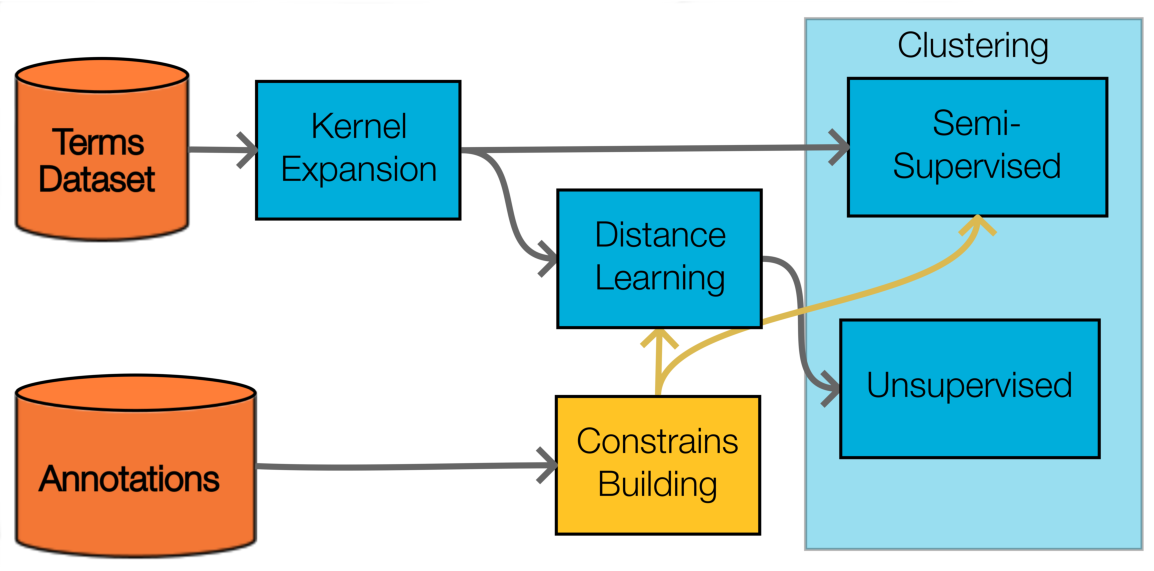
\includegraphics[width=0.95\columnwidth]{img/ANEW/scheme4.pdf}
  \caption{Block diagram of the clustering approach}
  \label{fig:ANEWblockdiag}
 \end{figure} 

Figure \ref{fig:ANEWblockdiag} shows the scheme of this work. We discuss the collection and generation of the annotated data and the building of the constraints to embed semantics about music in the learned distance metrics. We provide some quick details on the kernel expansion and distance learning techniques, since a more extensive description was presented in Sections \ref{sec:ML:kernels} and \ref{sec:ML:dist}, respectively. We then present the clustering techniques and the numerical results on the resulting clusters. Finally, we draw some overall considerations on the work.
%

In the following discussion, we will refer to \textit{emotion} and \textit{mood} as synonyms, as it is sometimes done in the natural language. It is worth remembering, however, that the two terms have different meanings. In \cite{Beedie2005} the authors investigate the difference between the meaning of the two terms by means of questionnaire proposed to non-academia participants and by reviewing the research works of the relating literature. The authors identify sixteen high-order themes of difference, such as \textit{duration} (moods have a generally considered to last longer),  \textit{awareness of cause} (the emotion is usually solicited by an identifiable source, while mood is often inexplicable), or \textit{display} (moods are considered rather personal, while emotions are more easy to be identified from an external observer). It is therefore hard to define a unique distinction between the meaning of the two terms. We will use \textit{mood} as a synonym of \textit{emotion} and, therefore, we will refer to the meaning of the latter for both terms.

\begin{table}[tb]
\caption{Summary of the collected data}
\label{tab:ANEWdata}
\begin{center}
\bgroup
\def\arraystretch{1.5}
\begin{tabular}{ ||p{.12\columnwidth} |l |p{.13\columnwidth}  |p{.50\columnwidth}||}
% \hline
\hline
\hline
Type &  Symbol & Num Terms & Details \\
\hline
\hline
Terms Dataset  &$\mathcal{D}_{\text{ANEW}} $ %=\{\mathbf{w}_1, ..., \mathbf{w}_N\}$
& 2,476 & Mean in V, A, D dimensions\\
% \hline
\hline
Implicit Distance  &$\mathbf{D}_{\text{ILM10K}}$& 240; 450 & Tag compact representation from an LSA with $k=10,20,50,100$ components\\
\hline
Explicit Distance  & $\mathbf{D}_{\text{HD}} $ & 180 & Human annotation of semantic similarity between terms from ANEW\\
\hline
Explicit Clustering  & $\mathbf{M}_{\text{HC}} $ & 100 & Human clustering of a subset of ANEW\\
\hline
\hline
% \hline
\end{tabular}\quad
\egroup
\end{center}
\end{table}


\subsection{Collection of the dataset}\label{sec:ANEW:data}
In this section, we describe three datasets created to provide the constraints for distance learning as well as to validate our approach. A summary of the collected data is provided in Table \ref{tab:ANEWdata}.

\subsubsection{Terms in the ANEW Dataset}
The terms in the ANEW dataset \cite{Bradley1999} are already annotated for the Valence, Arousal and Dominance dimensions with a value between 0 and 10 by psychology class students. We will refer to the ANEW dataset as
\begin{equation}
\mathcal{D}_{\text{ANEW}}=\{\mathbf{w}_1, ..., \mathbf{w}_T\}
\label{eq:ANEW:ANEW}
\end{equation} 
with $\mathbf{w}_i=\{\mu_V, \mu_A, \mu_D \}$, where $\mu_V$, $\mu_A$ and $\mu_D$ are the normalized average (between 0 and 1) of the annotations for the Valence, Arousal and Dominance descriptors respectively, and $T=2476$ is the number of terms in the ANEW dataset.  Specifically, we will refer to $\mathcal{D}_{\text{ANEW}}^{(VA)}$ and $\mathcal{D}_{\text{ANEW}}^{(VAD)}$ as the dataset with only Arousal and Valence dimensions considered and the dataset with also Dominance considered, respectively. 

\subsubsection{Implicit Distance Annotation}\label{sec:ANEW:ILM}
In Section \ref{sec:HLFs:LSA} we explained how we can perform  Latent Semantic Analysis (LSA) on an annotated dataset in order to infer a dimensional semantic space, which defines a metric of similarity among songs or terms. In this study, we compute a distance matrix among emotion related descriptors by performing LSA on a dataset composed of 10,199 tracks annotated with editorial and crowd sourced social tags, named I-Like-Music dataset, or ILM10K \cite{Saari2015, Allik2016}.
The dataset is annotated with weights corresponding to the prevalence of each tag in each song description. 

From the tags in ILM10K, we first discard the tags that are not included in the ANEW dataset. We then filter the tags that are rarely used by thresholding the frequency with which the tag  was used in ILM10K. We empirically choose the two thresholds as $15$ and $5$ times, leading to a set of $T=240$ and $T=450$ terms respectively. The former vocabulary contains less terms, but it is more reliable since they have been used quite often, while the latter is richer but the carried information might be less relevant. 

We build two tag-track matrices for the two sets $T=240$ and $T=450$, i.e., two matrices $\mathbf{A}_{\text{ILM10K}}^{(240)} \in \mathbb{R}^{240 \times 10199} $ and $\mathbf{A}_{\text{ILM10K}}^{(450)} \in \mathbb{R}^{450 \times 10199} $, respectively. We compute the $k$-component approximation of each matrix via LSA. We keep different numbers of components $k=10, 20, 50, 100$ to test different degrees of approximation, and we produce eight matrices $\mathbf{A}_{\text{ILM10K}}^{(T,k)} \in \mathbb{R}^{T \times k} $, one matrix for each combination of $T$ and $k$. 
 
Given a generic approximated matrix $\mathbf{A}_{\text{ILM10K}}$ (i.e., neglecting the notation about $T$ and $k$ for the sake of clarity), we compute two distance matrices between tags, using the Euclidean distance between the corresponding rows, producing the matrix  $\mathbf{D}_{\text{ILM10K}}$, and between the normalized rows (i.e.  $\mathbf{\tilde{A}}_{\text{ILM10K}}$), producing the matrix $ \tilde{\mathbf{D}}_{\text{ILM10K}}$. The latter matrix can be seen as a kind of transformation of the distance matrix using the Cosine-like distance. 

This procedure can also be interpreted as a Principle Component Analysis (PCA) \cite{Kim2005} and in fact PCA and LSA are two applications of the Singular Value Decomposition. From a (cleaned) tag-track matrix, we identify the $k$ principle linearly independent components from a linear combination of the $10,199$ tracks over the tag space. This procedure allows us to infer the similarity among tags from their use in the annotation task. 

\subsubsection{Human Distance Annotation}
\label{sec:ANEW:HDA}
We conducted an online survey to collect information on how people think of and rate the actual semantic similarity among emotional-related descriptors in the music context. We composed a subset of $T=240$ terms from the ANEW dataset as described in the previous Section \ref{sec:ANEW:ILM}. Each participant was asked to define the perceived emotional similarity in the context of music between pairs of descriptors with a value between $0$ (not similar at all) and $1$ (very similar). The pairs of descriptors proposed to the participants were randomly picked from the $T(T-1)/2$ possible combinations. We collected  
the received annotations and we inverted the score so that $0$ becomes the value for maximum semantic similarity and vice versa, in order to make the annotations consistent with the data described in Section \ref{sec:ANEW:ILM}. 

It is worth highlighting that the ANEW dataset collects annotation on the positions of emotional-related descriptors in the VAD space and the semantic similarity among terms is inferred by defining a metric of distance among the corresponding positions. The Human Distance Annotation aims to collect such semantic similarities by asking participants to explicitly annotate them.

504 people, either native or fluent English speakers, participated in the survey. Due to the high-number of possible pairs of terms, only a subset of them was annotated. In order to make the annotation more robust and reliable, we considered the pairs that received at least 2 annotations and the terms that belong to such pairs, leading to $T=180$. With the collected annotations, we compose the sparse matrix $ \mathbf{D}_{\text{HD}}$.

\subsubsection{Human Clustering Annotation}
\label{sec:ANEW:HCA}
Since we evaluate our approach by clustering the terms in the ANEW dataset in the original and new space, we also collected data on how people organize and group the emotional-related descriptors.

Therefore, we conducted a second online survey and asked annotators to group a subset of emotional-related descriptors. We selected a small subset of $T=100$ descriptors, in order to ease the cognitive load required for the manual grouping of the terms. The subset was composed of the most used tags in the ILM10K dataset. 

During the survey, we did not provide a fixed number of clusters, nor any suggestion or guideline, in order to collect the most possible unbiased annotations. At first, the participants were presented with the list of $100$ descriptors and an empty list of clusters. Testers were able to create as many clusters as they felt to need for their organization. 

$15$ people participated in the online survey, leading to the matrix $\mathbf{M}_{\text{HC}} $ with $T=100$ terms, where each entry $(i,j)$ indicates the number of people that grouped together the $i$-th and $j$-th terms. 

The number of participants that conducted the second survey is sensibly lower with respect to the first survey on the distance annotation. This is probably due to the high cognitive load of the task and the impossibility to use partially-annotated information. However, the information provided by $\mathbf{M}_{\text{HC}}$ is actually rich enough for the scope of our work. Indeed, while the matrix $ \mathbf{D}_{\text{HD}}$ is a sparse matrix, i.e., some pairs of terms might have not received any annotation, the matrix $\mathbf{M}_{\text{HC}} $ is a full matrix. Whenever $\mathbf{M}_{\text{HC}}(i,j)=0$, we can infer that all the $15$ participants have annotated that the $i$-th and $j$-th terms are too semantically dissimilar to be grouped in the same cluster. 

Please note that we refer to the annotations on clustering as $\mathbf{M}_{\text{HC}}$ since it indicates a similarity matrix, where the higher $\mathbf{M}_{\text{HC}}(i,j)$, the higher the similarity between the $i$-th and $j$-th terms, while we define $\mathbf{D}_{\text{HD}}$ and $\mathbf{D}_{\text{ILM10K}}$ as distance matrices.

\begin{figure}[bt] 
  \centering 
  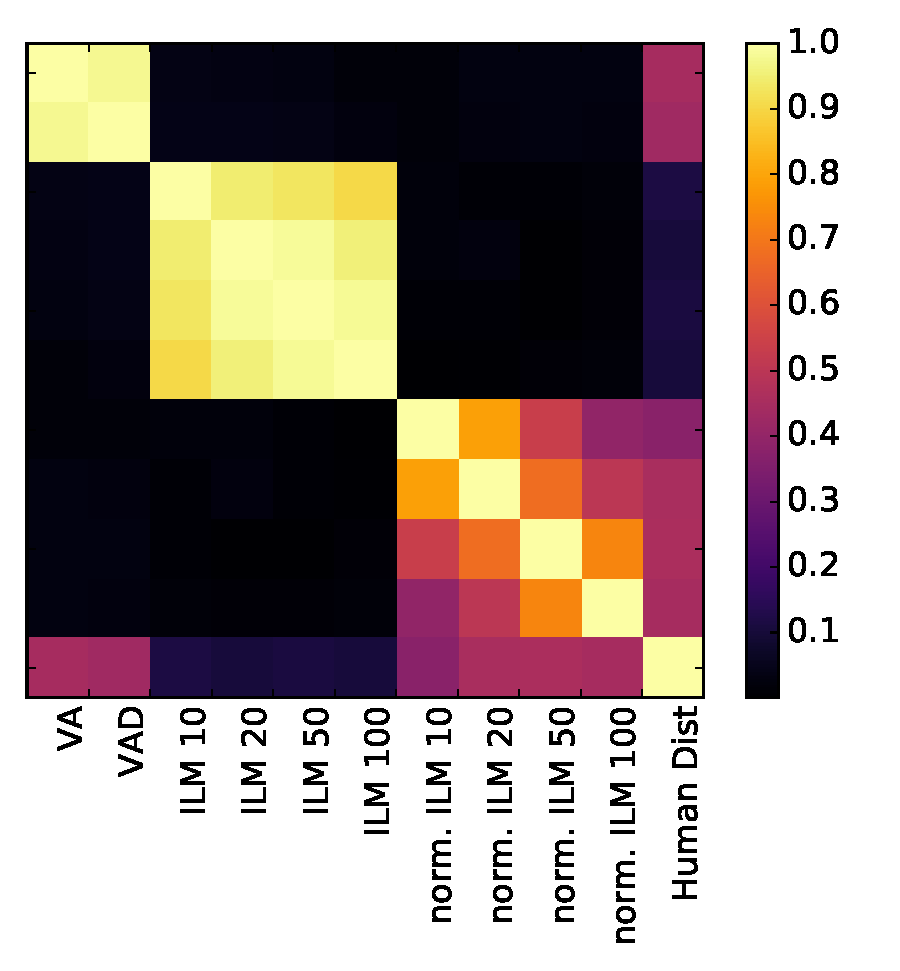
\includegraphics[width=0.80\columnwidth]{img/ANEW/pearson_dist_3.pdf}
  \caption{Absolute Pearson Correlation between the values of the distance matrices computed or collected from different sources of data.}
  \label{fig:ANEWdistData}
\end{figure}  

\subsubsection{Preliminary considerations on data}
We perform a preliminary statistical analysis of the collected data. We compute two self-distance matrices from the datasets $\mathcal{D}_{\text{ANEW}}^{(VA)}$ and $\mathcal{D}_{\text{ANEW}}^{(VAD)}$ using the Euclidean distance. We also consider the matrices computed or collected in Section \ref{sec:ANEW:data}, considering, for the ILM10K dataset, only $T=240$, since they are the most robust annotations. Finally, for each combination of pairs of matrices, we compute the absolute Pearson correlation between the values of the two matrices. In the case of the matrix $\mathbf{D}_{\text{HD}}$, which is sparse, we only considered the actual data of the matrix in the computation of the Pearson correlation. In Figure \ref{fig:ANEWdistData} we show the absolute Pearson correlations between the self-distance matrices from different sources of data we collected. 

We can see that there is absolutely no correlation between the Euclidean distance defined in the VA or VAD space and the one that can be inferred from the LSA of the ILM10K dataset. Moreover, it exhibits a modest correlation also with the human distance annotation. This confirms the need of a new space for the ANEW dataset which is more relevant for the music description.

\subsection{Learning the high-dimensional semantic space}
\label{sec:ANEW:moodtag}
In \cite{Barthet2013DesignAE} the authors investigate the existent semantic mood models for music recommendation and assess that two or three dimensions are not sufficient to producing a discriminative space for large music libraries. For this reason, we aim at producing a new space for the ANEW dataset by exploiting high-dimensional transformations of the VA or VAD space. In order to do this, we employ kernel expansions and distance learning techniques, as presented in Sections \ref{sec:ML:kernels} and \ref{sec:ML:dist}.

With respect to the techniques of kernel expansion, we employ the polynomial (degree 2 and 3) and RBF kernels described in \ref{sec:ML:kernels} in their explicit form. We also consider two non high-dimensional cases:
\begin{itemize}
\item we use the simple data in $\mathcal{D}_{\text{ANEW}}$ as-is, in order to take into consideration the non-expanded case and compare the new space with the traditional VA or VAD space;
\item we make use of the $L^2$ normalized data, by composing the dataset $\tilde{\mathcal{D}}_{\text{ANEW}}$ with the terms $\{\tilde{\mathbf{w}}_1,..., \tilde{\mathbf{w}}_T \}$, where each term is the $L^2$-normalization of the terms in $\mathcal{D}_{\text{ANEW}}$, i.e., 
\begin{equation}
\begin{split}
\tilde{\mathcal{D}}_{\text{ANEW}} &=\{ \frac{\mathbf{w}_1}{||\mathbf{w}_1||},..., \frac{\mathbf{w}_T}{||\mathbf{w}_T||}  \}\\
&=\{\phi(\mathbf{w}_1), ..., \phi(\mathbf{w}_T)   \},
\end{split}
\end{equation}
with the terms defined in Equation \ref{eq:ANEW:ANEW}.
\end{itemize}

With regard to the distance learning techniques, we employ the discussed techniques \cite{Carey2015}, i.e., Iterative Projection\cite{xing2003distance} (IP); Relevant Components Analysis \cite{bar2003learning} (RCA); Neighborhood Components Analysis \cite{goldberger2004neighbourhood} (NCA). We use the distance learning techniques to learn the subspaces defined by $\mathbf{L}$, with $\mathbf{L}\T \mathbf{L}=\mathbf{A}$ the Mahalanobis matrix, in order to find the (possibly) high-dimensional emotional space as a mapping: $\mathbf{L} \cdot \phi ( \mathbf{w}_t) $ with $t=1,...,T$. As discussed in Section \ref{sec:ML:dist}, in order to train the distance learning techniques we require a set of constraints as two sets of samples Must-Link $ML$ and Cannot-Link $CL$; the former indicate which samples must be placed together and the latter indicate which samples should be placed far apart. In the following Section, we explain the procedure we used to create such constraints.

\subsubsection{Constraints Building}
\label{sec:ANEW:constraints}
We build different sets of constraints from each implicit or explicit annotations we presented in Section \ref{sec:ANEW:data}.

Firstly,  we compute the ML and CL constraints from the ILM10K dataset (Section \ref{sec:ANEW:ILM}) by thresholding the values in the (possibly normalized) distance matrices $\mathbf{D}_{\text{ILM10K}}^{(T,k)}$, for every $T=\{240; 450\}$ and $k=10,20,50,100$. We first compute the mean value $\mu_{\text{ILM10K}}^{(T,k)}$ and standard deviation $\sigma_{\text{ILM10K}}^{(T,k)}$ of the values.
Given the generic matrix $\mathbf{D}_{\text{ILM10K}}$ , we define the two thresholds as $th_l= \mu_{\text{ILM10K}} - 2 \sigma_{\text{ILM10K}} $, $th_h= \mu_{\text{ILM10K}} + 2 \sigma_{\text{ILM10K}} $ (we neglect the notation of the matrix on the threshold for the sake of clarity).  We compose the set of ML constraints by considering those pairs of terms which are close in the space defined by LSA, hence whose distance is lower than $th_l$, and the CL set with those pairs of terms that are far from each other, i.e., whose distance is higher than $th_h$, i.e.:
\begin{equation}
ML=\{ (i, j) : \mathbf{D}_{\text{ILM10K}}(i,j)<th_l    \};
\end{equation}
\begin{equation}
CL=\{ (i, j) : \mathbf{D}_{\text{ILM10K}}(i,j)>th_h    \}.
\end{equation}
We compose the same sets of constraints from the normalized matrices $\mathbf{\hat{D}}_{\text{ILM10K}}$.

We use a similar approach to compose the ML and CL constraints from the Human Distance annotations. We compute the mean value $\mu_{\text{HD}}$ and standard deviation $\sigma_{\text{HD}}$ of the annotations in the matrix $\mathbf{D}_{\text{HD}}$ and we empirically define the thresholds $th_l=\mu_{\text{HD}} - \sigma_{\text{HD}},\; th_h=\mu_{\text{HD}} + \sigma_{\text{HD}}$ . In this case, the value of $\sigma_{\text{HD}}$ is higher than the ones obtained from the ILM10K distance $\sigma_{\text{ILM10K}}$, and therefore we choose a softer threshold and we do not use $2 \sigma_{\text{HD}}$.

Finally, from the Human Clustering annotations we compute the mean value $\mu_{\text{HC}}$ and standard deviation $\sigma_{\text{HC}}$ of the non-zero entries of the matrix $\mathbf{M}_{\text{HC}}$, i.e., of the number of people who annotated two terms as belonging to the same clusters, and define the soft threshold $th= \mu_{\text{HC}} - \sigma_{\text{HC}} $. We compose ML with the pair of terms that have been grouped together by more than $th$ people and we compose CL with the zero entries of $\mathbf{M}_{\text{HC}}$.

\subsection{Experimental setup}
\label{sec:ANEW:results}
As previously discussed, our aim is to find a transformation of the ANEW space with improved conceptual organization of terms that is relevant in a musical context. We expect terms that are semantically similar in this context to be close and dissimilar terms to be far apart. For this reason, we validate our approach by clustering the ANEW dataset in the transformed spaces. We employ some of the techniques described in Section \ref{sec:ML:clust}, specifically:
\begin{itemize}
\item the K-means algorithm  \cite{macqueen1967some};
\item the Spectral Clustering (SC) algorithm \cite{shi2000normalized};
\item the Agglomerative Hierarchical Clustering (AHC) algorithm \cite{sibson1973slink};
\item the Semi-Supervised Non-Negative Matrix Factorization (SS-NMF) algorithm \cite{chen2008} .
\end{itemize}

%A clustering algorithm is a machine learning technique that aims at grouping together the samples that are close together in a given space, where their distance is defined by some metric. In order to provide a robust evaluation, we apply several clustering techniques: the K-Means, the Semi-Supervised Non-Negative Matrix Factorization, the Spectral Clustering and the Agglomerative Hierarchical Clustering.

%The K-Means \cite{macqueen1967some} is a common unsupervised clustering algorithm, which first defines a centroid for each cluster and then assigns the samples to the closest centroids, i.e., to the correspondent cluster. The position of the centroids are adjusted to be the actual centroid of the assigned samples and the assignment is ran again. This two steps procedure is ran for several iterations until convergence. While K-Means algorithm is effective to retrieve clusters with a globular shape \cite{PAMI} (i.e., with similar variance in all the dimensions), the distance learning techniques can provide a better separation of clusters and address the issue.

%The Semi-Supervised Non-Negative Matrix Factorization \cite{chen2008} (SS-NMF) applies the Non-Negative Matrix Factorization discussed in Section \ref{sec:ML:MSA} for the case of Music Structure Analysis. The NMF is able to decompose a matrix into a sum of components; in this case, the self-distance matrix of the terms in the new space is factorized in order to retrieve the main components, i.e., the main clusters. 

%The Spectral Clustering \cite{shi2000normalized} (SC) technique was also presented in Section \ref{sec:ML:MSA}. As mentioned, a graph is built from the distance matrix, with the nodes given by the samples and the edges defined by the (possibly learned) distances between them. The SC technique looks for the lowest cost partition of the graph, by employing a low-dimension reduction of the distance matrix and applying the K-Means algorithm on it.

%Finally, Agglomerative Hierarchical Clustering \cite{sibson1973slink} (AHC) follows a bottom-up approach to build the clusters. At the first iteration, each sample is a separate cluster. Then, the two closest clusters merge together as a cluster with two samples. The clusters keep merging until the desired number of clusters is reached. 

%Clustering the samples is commonly a unsupervised task. However, some algorithms can be adapted to be trained in a semi-supervised fashion, as described in Section \ref{sec:ML:clust}. 
We use the SS-NMF, SC and AHC techniques with both the unsupervised and semi-supervised  approach, while using K-means with the purely unsupervised fashion, as explained in Section \ref{sec:ML:clust}.

%are able to include some apriori information by processing the distance matrix with some constraints. Given the generic distance matrix $\mathbf{M}$ and two sets of constraints $CL$ and $ML$ as defined above, we can include the constraints by computing the matrix $\mathbf{D}$ as:
%\begin{equation}
%\mathbf{D}=[\mathbf{M}(i,j)- \zeta_{i,j} + \vartheta_{i,j}] 
%\end{equation}
%where $\zeta_{i,j}\geq 0$ if $(i,j)$ is in the $ML$ set and $\vartheta_{i,j}\geq 0$ if $(i,j)$ is in the $CL$ set. This makes the samples in the $ML$ set closer and the samples in the $CL$ set further apart. In this work we empirically choose a constant value for all the distances, equal to half the range of the values in the matrix $\mathbf{M}$.

%In this study we use the SS-NMF, SC and AHC algorithms in both unsupervised and semi-supervised fashion. 

In order to validate the actual contribution of the distance learning techniques, we compare the results of our approach with the results obtained with both unsupervised and semi-supervised clustering of the ANEW dataset. Hence, we have three scenarios: 
\begin{enumerate}
\item the unsupervised clustering of the transformed (but not learned) space (\textbf{Unsup.});
\item the semi-supervised clustering of the transformed (but not learned) space (\textbf{SemiSup.}); 
\item our approach, that is the unsupervised clustering of the learned space (\textbf{Dist. Learn}).
\end{enumerate} 
It is worth remembering that the first scenario also includes the clustering of non-transformed space using the Euclidean distance. 

We perform the clustering over all the combinations of input, kernel expansion, constraints, distance learning and clustering techniques. Given the large number of configurations we need to test, we experimentally choose to retrieve the $6$ best representative clusters. In the following Section, we present the evaluation of the obtained clusters.

\subsection{Numerical results}
Since we have several configurations to test, and we do not have a full ground truth on the problem of clustering, we validate our approach by performing three different evaluations:
\begin{enumerate}
\item we use the objective metric called Silhouette index (Section \ref{sec:ANEW:obj_results}, Fig. \ref{fig:ANEWsilhouette}, Table \ref{tab:ANEWsilhouette}),  which perform a qualitative evaluation of the relation between the input data and the resulting clusters;
\item we compare the obtained clusters with the clustering of the samples defined by the rows of $\mathbf{D}_{\text{ILM10K}}$, in order to validate the degree of similarity between the clustering in the new space and the clustering in a space defined by music annotations (Section \ref{sec:ANEW:subILM10K_results}, Fig. \ref{fig:ANEWILM10K}, Table \ref{tab:ANEWv_score});
\item we compare the obtained clusters with the human annotation of clustering described in Section \ref{sec:ANEW:HCA} (Section \ref{sec:ANEW:subHC_results}, Fig. \ref{fig:ANEWF_measure}, Table \ref{tab:ANEWf_measure}).
\end{enumerate}

In the following, we separately discuss the three kinds of evaluation.

\begin{table}[tb]
	\caption{Best results for the Silhouette Index for each scenario}
	\label{tab:ANEWsilhouette}
%    \small
\begin{center}
  \bgroup
  \def\arraystretch{1.5}
\begin{tabular}{ ||l |l |l |l  |c||}
\hline
\hline
% \hline
Scenario & Features & Algorithm & Constraints & Silhouette \\
\hline
\hline
Unsup. & Norm. VA & kmeans & & 0.5287 \\
\hline
Semi-Sup. & Norm. VA & SC & $\mathbf{{M}}_{\text{HC}}$ & {\color[HTML]{8E0000} \textit{0.5240}} \\
\hline
IP Dist. & VAD & kmeans & $\mathbf{{D}}_{\text{HD}}$  & 0.5432 \\
\hline
RCA Dist. & VAD, poly 3 degree & AHC & $\mathbf{{M}}_{\text{HC}}$ & {\color[HTML]{326B00}  \textbf{0.6864}} \\
\hline
NCA Dist. & VA, poly 2 degree & kmeans & $\mathbf{\hat{D}}_{\text{ILM10K}}$, $T=240$, $k=10$ & 0.5456 \\
\hline
\hline
\end{tabular}\quad
\egroup
\end{center}
\end{table}



\begin{figure}[tbph]
  \centering 
  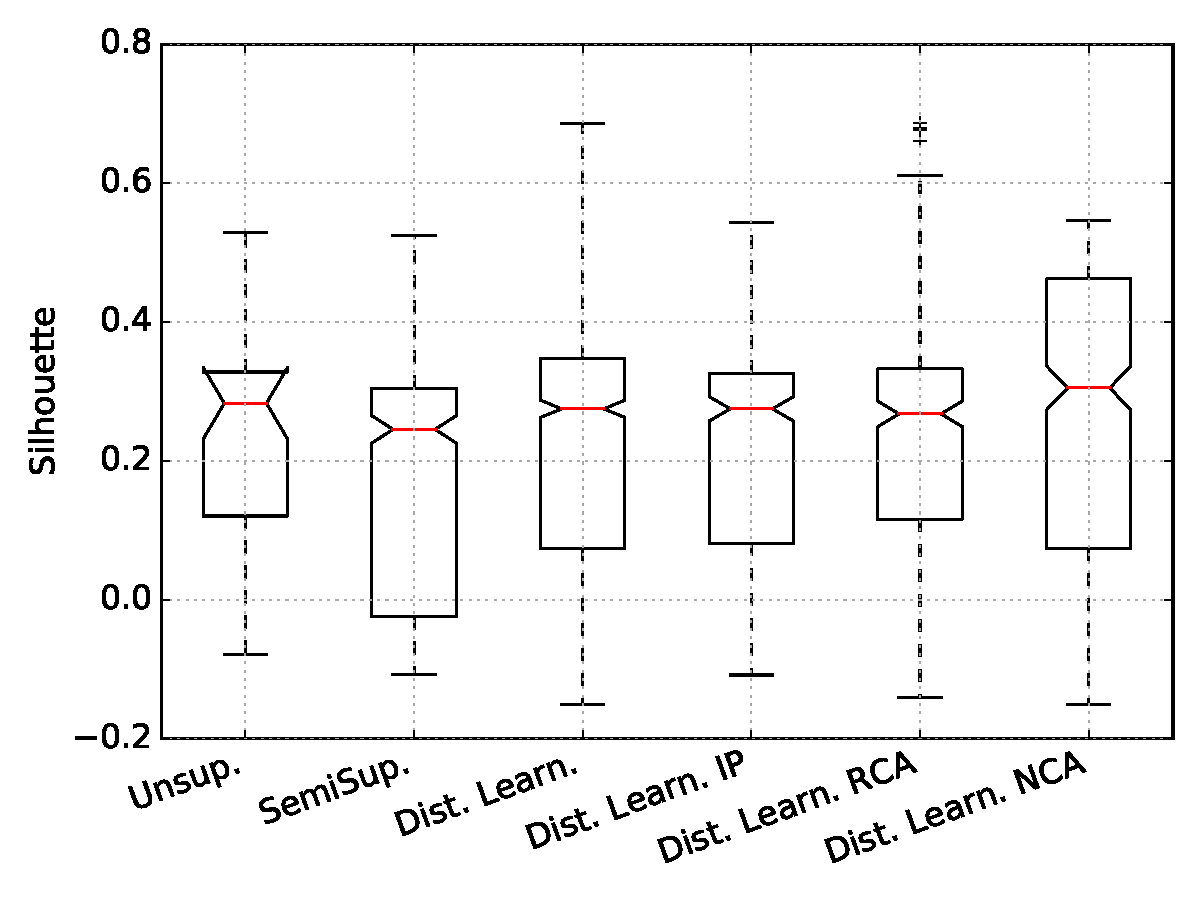
\includegraphics[width=0.85\columnwidth]{img/ANEW/Silhouette2.pdf}
  \caption{Boxplot of the Silhouette indices for the different scenarios}
  \label{fig:ANEWsilhouette}
\end{figure}  


\subsubsection{Objective metrics} \label{sec:ANEW:obj_results}
The Silhouette index is an objective quality metric that defines how much the clusters are compact and well separated. In order to do so, it defines for each sample $s$ a variable $a$ as the mean distance to all the samples in the same cluster and a variable $b$ as the mean distance to all the samples in the next nearest cluster. In order for a clustering to be well separated, $a$ should be small and $b$ should be high. The Silhouette index is hence computed as \cite{scikit-learn}:
\begin{equation}
\text{Silhouette}=\frac{1}{|\mathcal{D}|} \sum_{s \in \mathcal{D}} \frac{b-a}{\text{max}(a,b)}\in [-1,1],
\end{equation}
where $\mathcal{D}$ is the generic dataset of samples.  High (positive) values of Silhouette indicate dense well-separated clusters, values around $0$ indicate overlapping clusters and low (or negative) values indicate incorrect clusters. 

In Figure \ref{fig:ANEWsilhouette} we show the boxplots of Silhouette metric for the different scenarios, while in Table \ref{tab:ANEWsilhouette} we show the configurations that generate the best results for each scenario. 

It is clear that the application of Distance Learning techniques outperforms unsupervised and semi-supervised techniques, even with different configurations of kernels, algorithms and constraints. In particular, the best performance is obtained with the Agglomerative Hierarchical Clustering over the third degree polynomial expansion of the VAD dataset, with a translation learned using the RCA technique constrained by the data collected from the Human Clustering. 

From the boxplot we can see that the RCA distance learning presents some extremely high values of Silhouette, which are considered outliers. Nevertheless, even without the supposed-outlier configurations, the RCA technique achieves the highest results for the Silhouette index, while the NCA technique achieves the highest average result over the different configurations. 

We can also notice that the semi-supervised scenario performs on average worse than the unsupervised scenario. This is because the Silhouette index evaluates the resulting clusters with respect of the position of the input data, that is not moved from the original position. The estimated clusters are therefore more noisy, which confirms the advantage of distance learning techniques to transform the space.


\begin{figure}[tbp]
  \centering %\includegraphics[width=0.75\columnwidth]{img/ANEW/ILMVscore.pdf}
 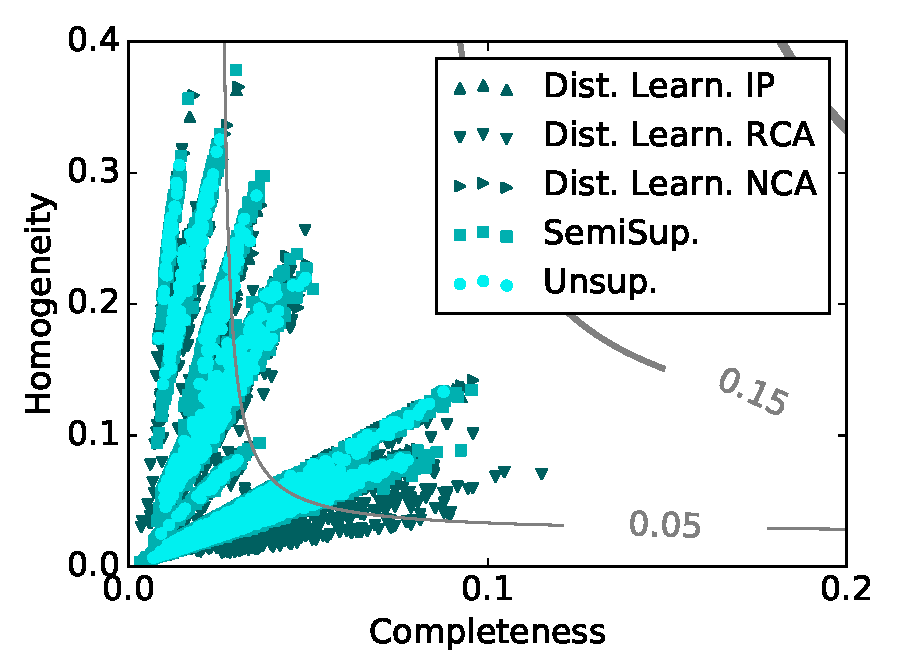
\includegraphics[width=.85\columnwidth]{img/ANEW/ILMVscore_square.pdf}
  \caption{Completeness and Homogeneity results for the comparison of clusters with those obtained from the ILM10K dataset. Gray contour lines indicate the V-score}
  \label{fig:ANEWILM10K}
\end{figure}


\subsubsection{Subjective metrics - Comparison with Clustering of ILM10K}
\label{sec:ANEW:subILM10K_results}
Our proposed approach aims to draw from the ANEW dataset a new high-dimensional space that bears more relevance for the music annotation. In this regard, we compare the clusters obtained with the different approaches with clusters obtained directly from a music annotation scenario. In order to do so, we rely on the data inferred from the ILM10K dataset and apply the aforementioned unsupervised clustering techniques to the samples of $\mathbf{A}_{\text{ILM10K}}^{(T,k)}$ and $\mathbf{\tilde{A}}_{\text{ILM10K}}^{(T,k)}$ for the different $T$ and $k$. In this case, we have a set of predicted clusters and a set of ground truth clusters, and we want to estimate how much the former resembles the latter.  

We consider the homogeneity and completeness metrics \cite{rosenberg2007v}. The two metrics range between 0 and 1, and higher values correspond to better performance. More specifically, the homogeneity metric evaluates whether each estimated cluster contains only members of a group in the ground truth, while the completeness metric, instead, estimates whether the samples of a given group belongs to the same estimated cluster. The homogeneity and the completeness metrics are computed from the conditional entropy of the classes given the cluster assignment $H(C|K)$ and from the conditional entropy of clusters given class $H(K|C)$, respectively:
$$
	\text{homogeneity}=1-\frac{H(C|K)}{H(C)},
$$
$$
\text{completeness}=1-\frac{H(K|C)}{H(C)},
$$
with 
$$
H(C|K)=-\sum_{c=1}^{|C|}\sum_{[k=1]}^{|K|} \frac{n_{c,k}}{n} \log (\frac{n_{c,k}}{n_k}),
$$
$$
H(K|C)=-\sum_{c=1}^{|C|}\sum_{[k=1]}^{|K|} \frac{n_{c,k}}{n} \log (\frac{n_{c,k}}{n_c})
$$
the aforementioned conditional entropies and
$$
H(C)=-\sum_{c=1}^{|C|} \frac{n_c}{n} \log(\frac{n_c}{n}),
$$
$$
H(K)=-\sum_{k=1}^{|K|} \frac{n_k}{n} \log(\frac{n_k}{n}),
$$
the entropy of clusters from ground truth or estimation respectively, with $|K|$ the number of estimated clusters, $|C|$ the number of ground-truth groups, $n_c$ and $n_k$ the number of samples that belong or are assigned to the cluster $c$ or $k$, respectively, and $n_{c,k}$ the number of samples belonging to the $c$-th cluster and assigned to the $k$-th's one.
We also consider the V-measure, i.e., the harmonic mean of homogeneity and completeness. 

To avoid overfitting issues, we do not consider those configurations that are trained with the constraints generated from the ILM10K dataset. More specifically, we evaluate only the configurations generated from the expanded VA and VAD dataset using either distance learning techniques or semi-supervised clustering techniques with constraints generated from the Human Distance or Human Clustering annotations.


We show the distribution of results for the different scenarios in Figure \ref{fig:ANEWILM10K}, where each point is a different configuration. We can visually estimate there are some stripes in the distribution of results, which are probably caused by the different sets of ground truth generated by the different clustering techniques and datasets from the ILM10K dataset. 
We notice the results are fairly low, showing that the organization given by the expanded and possibly learned ANEW dataset is very different from that inferred from social tags on a real music annotation scenario. This confirms the low correlation shown in Figure \ref{fig:ANEWdistData} and the necessity to find a space for the ANEW dataset which is more useful for MIR applications. However, it is clear that our approach can only slightly improve the task. 


\begin{table}[tbp]
	\caption{Best results of the Homogeneity, Separation and V-measure metrics for the comparison with the clusters generated by the AHC from the normalized ILM10K dataset ($T=240$, $k=100$)}
	\label{tab:ANEWv_score}
    \small
\begin{center}
  \bgroup
  \def\arraystretch{1.5}
\begin{tabular}{ ||l  |l| l |l  |c|c|c ||}
\hline
\hline
Scenario    & Features    &  Alg.   & Constr.   & Compl.  & Hom.  & V-score \\
\hline
\hline
Unsup.  & VA, poly 3 degree & SC &  &  0.0877 & 0.1334 & 0.1058 \\
\hline
Semi-Sup. & VAD poly 2 degree & AHC     & $\mathbf{{D}}_{\text{HD}}$   & 0.0955 & 0.1347 & 0.1118 \\
\hline
IP Dist. & VA       & SC    & $\mathbf{{D}}_{\text{HD}}$     & 0.0929 & 0.1371 & 0.1107 \\
\hline
RCA Dist. & VAD & kmeans & $\mathbf{{D}}_{\text{HD}}$ & 0.0869 & 0.1290 & {\color[HTML]{8E0000} \textit{0.1038}} \\
\hline
NCA Dist.& VA, poly 2 degree & AHC & $\mathbf{{D}}_{\text{HD}}$   & 0.0959 & 0.1421 & {\color[HTML]{326B00} \textbf{0.1145}}  \\
\hline
\hline
\end{tabular}
\egroup
\end{center}
\end{table}

In Table \ref{tab:ANEWv_score} we list the configurations that lead to the best performance. Such configuration are able to achieve a V-Score between $0.1058$ and $0.1145$, which is quite low. From the range of the best results in the Completeness and Homogeneity values, we can infer that the best results are all generated from the same configuration of the ILM10K ground truth, i.e., the one composed by the Agglomerative Hierarchical Clustering on the normalized dataset with 240 terms and $k=100$. This configuration is the most informative and reliable one, since it has few widely-used tags and the highest number of components, i.e., the richest approximation of the original matrix.  

Moreover, we can also see that all the highest results have been achieved by using the constraints from Human Distance. We believe that the reason of this is the medium-high correlation between the Human Distance annotation and the normalized ILM10K dataset, as shown in Figure \ref{fig:ANEWdistData}.

The best results is reached using NCA technique with a AHC over the polynomial-expanded VA dataset. We can see that the dataset and the kernel is the same that obtained the second highest result for the Silhouette metrics in Table \ref{tab:ANEWsilhouette} for the NCA technique. Moreover, the AHC is also used for the two highest results in this case, the NCA distance learning technique and the Semi-Supervised clustering.

However, since all the results are rather low, we cannot draw meaningful conclusions from this evaluation.

\subsubsection{Subjective metrics - Comparison with Human Annotations}
\label{sec:ANEW:subHC_results}
We finally compare the obtained clusters with those collected from human clustering annotations (HC). For this case, we will use traditional Precision, Recall and F-Measure metrics, which focus more on the the correctly grouped terms rather than the correctly non-grouped ones, since the former are more specific and relevant.

We define the matrix $\mathbf{Y}\in \mathbb{R}^{T \times T}$ of HC annotation as $\mathbf{Y}(i,j)=1$ if the $i$-th and $j$-th samples are in the same cluster by thresholding the matrix $\mathbf{M}_{\text{HC}}$ with $th=\mu-\sigma$, similarly as in Section \ref{sec:ANEW:constraints}. We then compose the matrix $\hat{\mathbf{Y}}$ from the estimated clustering results, and we define the sets $TP$, $FP$ and $FN$ as:
\begin{equation}
TP=\{(i,j) : \mathbf{Y}(i,j)=\hat{\mathbf{Y}}(i,j)=1 \};
\end{equation}
\begin{equation}
FP=\{(i,j) : \mathbf{Y}(i,j)\neq 1=\hat{\mathbf{Y}}(i,j) \};
\end{equation}
\begin{equation}
FN=\{(i,j) : \mathbf{Y}(i,j)=1 \neq \hat{\mathbf{Y}}(i,j) \}; 
\end{equation}
with $i,j=1,...,T$ and  $i<j$ to avoid duplicate pairs of samples such as $(i,j)$ and $(j,i)$. The Precision, Recall and F-Measure as \cite{Manning2008}: 
\begin{equation}\label{eq:HLFs:P}
P=\frac{|TP|}{|TP|+|FP|}\in [0,1];
\end{equation}
\begin{equation}\label{eq:HLFs:R}
R=\frac{|TP|}{|TP|+|FN|}\in [0,1];
\end{equation}
\begin{equation}\label{eq:HLFs:F}
F=\frac{2 P R}{P+R}\in [0,1].
\end{equation}
The Precision indicates the ratio of correctly clustered samples with respect to all the clustered samples; the Retrieval indicates the ratio of correctly clustered samples with respect to the samples that were supposed to be clustered together; the F-Measure is the harmonic mean between the two measures that provides a useful compact metric. The balanced F-measure, indeed, achieves high values only when both Precision and Recall are assigned with high values, while if either $P=0$ or $R=0$, we obtain $F=0$ regardless to the other metric.  

To avoid overfitting, we evaluate only configurations that are not trained with the constraints generated from the human annotations on clustering.

\begin{figure}[tbp]
  \centering 
     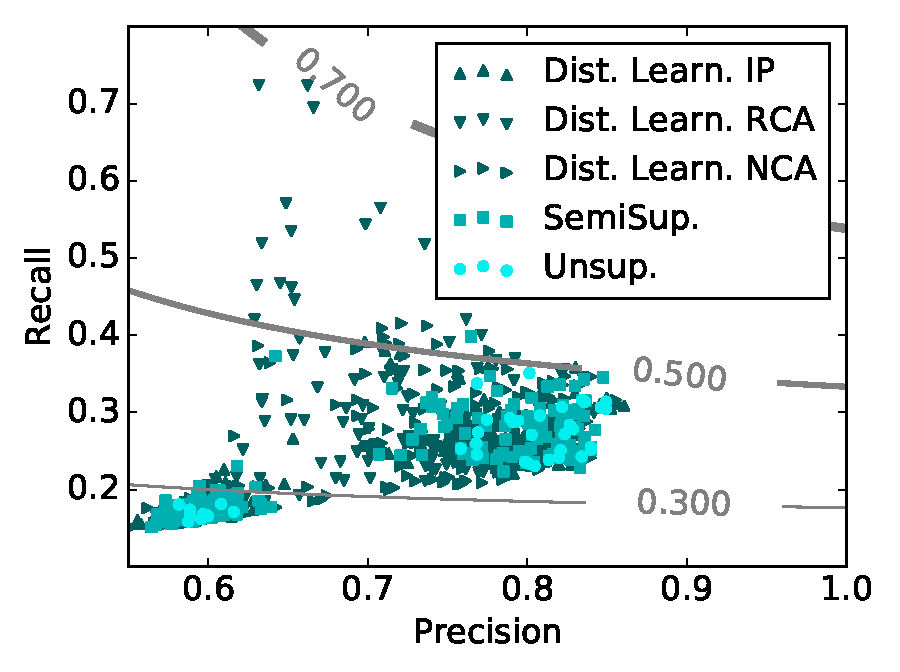
\includegraphics[width=.85\columnwidth]{img/ANEW/F_measure_square.pdf}
  %  \includegraphics[width=0.7\columnwidth,height=5cm]{img/ANEW/F_measure.pdf}    
  \caption{Precision and Recall results for the comparison of clusters with those obtained from human annotation. Gray contour lines indicate the F-measure.}
  \label{fig:ANEWF_measure}
\end{figure}  

In Figure \ref{fig:ANEWF_measure} we show the distribution of results for the different scenarios and configurations. In general, Precision is higher than Recall, showing that the estimated clustering is not capable of retrieving all the correct groups, while it is effective of correctly estimating the clusters. The F-measures are mostly distributed between 0.3 and 0.5, which is an average result. In particular, we can notice two notable trends, one around $P=0.6$ and one around $P=0.8$.
However, we can clearly see that some configuration from RCA Distance Learning are able to improve the average Recall and achieve highest values of F-measure.  The F-measure is achieved by losing some effectiveness in the Precision, leading to a rather balanced performance between $P$ and $R$. We can see that at least $9$ RCA configurations obtained higher results than any other configurations, and only one Semi-Supervised technique achieves $F>0.5$. This consideration clearly shows that the distance learning techniques are more effective to embed the information from constraints to better organize the terms with respect to the music context. 

\begin{table}[tb]
	
	\caption{Best results for the Precision, Recall and F-measure metric for the comparison with the human annotated clusters }
	\label{tab:ANEWf_measure}
\begin{center}
  \bgroup
  \def\arraystretch{1.5}
\begin{tabular}{ ||l |l| l |p{.15\textwidth} |c  |c|c||}
\hline
\hline
Scenario    & Features    &  Algorithm  & Constraints     & P   & R   & F \\
\hline
\hline
Unsup.  & VAD, RBF & kmeans     &          &  0.8012 & 0.3512 & {\color[HTML]{8E0000} \textit{0.4883}} \\
\hline
Semi-Sup. & VAD, RBF & AHC    & $\mathbf{{D}}_{\text{HD}}$     & 0.7646 & 0.3986 & 0.5240 \\
\hline
IP Dist. & VAD, RBF & AHC     & $\mathbf{\hat{D}}_{\text{ILM10K}}$, $T=240$,$\quad \;$ $k=100$ & 0.6979 & 0.3915 & 05016 \\
\hline
RCA Dist. & VA, poly 3 degree & AHC & $\mathbf{\hat{D}}_{\text{ILM10K}}$, $T=240$,$\quad \;$ $k=50$ & 0.6622 & 0.7241 & {\color[HTML]{326B00}  \textbf{0.6918}} \\
\hline
NCA Dist.& VAD, RBF & kmeans & $\mathbf{\hat{D}}_{\text{ILM10K}}$, $T=240$,$\quad \;$ $k=10$ & 0.7971 & 0.4124 & 0.5289  \\
\hline
\hline
\end{tabular}\quad
\egroup
\end{center}
\end{table}

In Table \ref{tab:ANEWf_measure} we list the best configurations for each scenarios. The RCA Distance Learning technique clearly outperforms the other approaches and matches very closely the human annotations, i.e., the way people organize the emotional-related descriptors. We can notice that once again, the best results are obtained by using the AHC over some polynomial expansion of the dataset. Moreover, all the distance learning techniques take advantage of the constraints generated from the most informative set of annotations, i.e., the normalized ILM10K dataset with fewer terms. In this scenario, however, lower components are required to achieve higher results: the RCA distance learning achieves its best results with $k=50$ components and the NCA distance learning with just $k=10$ components.

\subsection{Final remarks}\label{sec:ANEW:conclusions}

In this Section we investigated a possible formalization of the semantic domain as a dimensional semantic model for emotional-related descriptors. While the VA model and the ANEW space have been used in the MIR community for several years, this study proposed an useful approach to improve its ability of describing and possibly retrieving musical content by including information inferred from annotated dataset.

We introduced a novel approach consisting of kernel expansion, constraint building from task specific human annotation and finally distance learning to transform the ANEW dataset and obtain a distribution of terms that provides better conceptual organization with respect to the conventional VA or VAD spaces.

We validated our approach by evaluating its ability to conceptually organize the terms by performing some clustering techniques on the expanded and learned space, using subjective and objective evaluation metrics. We evaluated our proposed approach in a high-number of configurations, which we grouped into three main approaches: unsupervised clustering of the expanded space, semi-supervised clustering of the expanded space and unsupervised clustering of the learned expanded space. For each approach and for each metric we showed 
the average and the maximum results over the configurations. The average and maximum results prove that the use of distance learning techniques improves the position and therefore the organization of concepts of the ANEW dataset. In particular, agglomerative hierarchical clustering of a RCA-learned space based on the polynomial expansion of VA/VAD space outperforms the other configurations. 




\begin{figure}[bt] 
	\centering 
	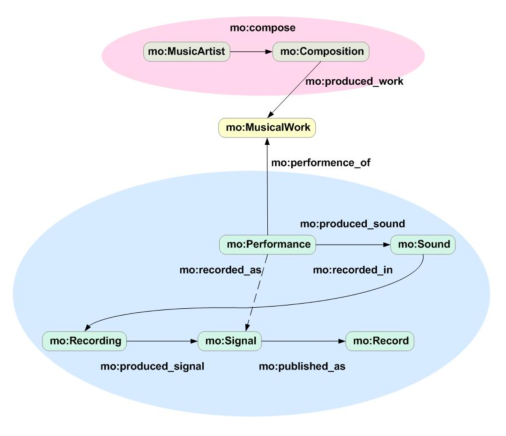
\includegraphics[width=\textwidth]{img/HLFs/ontology.pdf}
	\caption{An example of a definition in an ontology \cite{Raimond2007}}
	\label{fig:HLFs:ontology}
\end{figure}	

\section{Ontologies}\label{sec:HLFs:ontology}
In the formalization of the semantic domain, a semantic model can effectively tackle the complexity of the natural language, by defining the set of descriptors and their semantic relations. In principle, we would like to be able to model all the kind of relations among descriptors, such as the notion of "composition", or how the music genre is related to some emotion-based features. In order to formalize the semantic domain, we need in fact to model the full knowledge of music. 

In computer and information science, an \textit{ontology} is a structural framework that models the representation of knowledge as a set of concepts \cite{Bechhofer2009}. An ontology can model a richer information with respect to semantic models, because it allows to hierarchically organize the semantic domain. A subset of the knowledge defined by an ontology, can be modeled and defined as an ontology itself.

The ontologies are a promising step toward a full definition of the semantic domain, although they require a considerable effort and the literature has not yet defined a set of reliable automatic tools to define or populate it. In \cite{Raimond2007} the authors present an ontology for editorial, cultural and acoustic music information. In Figure \ref{fig:HLFs:ontology} we show the description of a music production work flow from \cite{Raimond2007}, which explicits the complexity of modeling an ontology. In \cite{Zanoni2014} the authors present an ontology for the formalization of the knowledge on violin instruments as a part of a wider ontology on bowed instruments, which we use to formalize a semantic model in Chapter \ref{Chap:Violin}. In \cite{ElRaheb2012} the authors introduce an ontology for representing dance movements.  

\section{Final considerations}
We provided an overview of  different approaches used in the MIR literature to formalize the semantic domain of the musical content, by means of high-level features. These approaches have different levels of complexity, depending on the problem addressed. We discussed the two main approaches for the more abstract and subjective description, i.e., the categorical and the dimensional approaches. We presented the categorical approach, that defines the semantic domain as a set of disjoint or overlapping categories. The categorical approach has however some limitations in its descriptive power, due to the graded descriptions of natural language. Moreover, due to the time variance of music, the description of entire songs is also limited. We provide an overview of the semantics of musical structure, which addresses the limitation regarding the time variance of music. We then address the graded description by discussing dimensional semantic models,  which overcomes the issues raised by the categorical approach based on discrete classes by allowing the model to represent the HLFs within a continuous range of values, and possibly define the semantics among terms. As a special case of semantic model, there are the widely used Valence-Arousal model for emotion representation and the Latent Semantic Analysis, to infer a semantic model from unstructured annotations such as those from social tags. 

With this regard, we investigated a novel hybrid approach for a semantic model, that enriches the manually annotated dataset in the Valence-Arousal space with prior information drawn from unstructured annotations, in order to build a more complete and accurate semantic model for emotion-related descriptors. We obtained several high-dimensional non-linear transformations of the manually annotated dataset, driven by the unstructured annotations of musical items, therefore tailoring the generic dataset to the specific sake of music description. 

Finally, we provided a brief overview of the ontologies, which are the most complex formalization for the semantic domain, since they are able to fully represent the knowledge on a specific topic, in this case, the high-level description of music.